\setcounter{rownumber}{0}
\chapter{Laser Cooling of Traveling-Wave Phonons in an Optical Fiber}
\label{ch:Cooling}
\acresetall

Joel N. Johnson\affil{Department of Applied Physics and Materials Science, Northern Arizona University, Flagstaff, AZ 86011, USA}%
\affil{Center for Materials Interfaces in Research and Applications, Flagstaff, AZ 86011, USA},
Danielle R. Haverkamp\affilmark{1}\affilmark{2},
Yi-Hsin Ou\affil{College of Optical Sciences, University of Arizona, Tucson, AZ, USA},
Khanh Kieu\affilmark{3},
Nils T. Otterstrom\affil{Photonic and Phononic Microsystems, Sandia National Laboratories, Albuquerque, New Mexico, USA},
Peter T. Rakich\affil{Department of Applied Physics, Yale University, New Haven, CT, USA},
Ryan O. Behunin\affilmark{1}\affilmark{2}

\hfill

\textit{This chapter elaborates on experiments and results related to the demonstration of optomechanical cooling of traveling-wave phonons in an optical fiber, which have been published as an article by the same name in Physical Review Applied by the author (Johnson et al. 2023).} \normalfont{\cite{johnson2023laser}} \textit{Any discrepancies, omissions, or errors that may exist between the published paper and this dissertation chapter are the sole responsibility of the author, as the text, analyses, and interpretations herein represent an independent and original presentation of the work.}

%--------------------------------------------------------------------%

\section{Introduction}
\label{Cooling:sec:Introduction}

Over the past half-century, light-based techniques have dramatically reshaped how we control mechanical motion. Laser cooling has become indispensable across many branches of physics, allowing researchers to reduce thermal motion in ions, atoms, and mesoscopic oscillators to previously unimaginable levels. From the earliest proposals and demonstrations of Doppler cooling in dilute gases \cite{hansch1975cooling} to the realization of ultracold quantum gases in Bose–Einstein condensates, \cite{anderson1995observation} the ability to reduce thermal motion with light has profoundly transformed \ac{AMO} physics, enabling breakthroughs ranging from high-precision atomic clocks to quantum state preparation. \cite{ludlow2015optical} Equally impactful is the extension of laser cooling concepts into solid-state systems. In rare-earth-doped optical crystals, for example, anti-Stokes fluorescence cooling has now approached cryogenic temperatures, cooling Yb-doped solids down to \(\sim\)\SI{87}{\kelvin} (the boiling point of liquid argon) and projected to reach \SI{77}{\kelvin} (liquid nitrogen) in the near future. \cite{meng2018realization} Such optical refrigeration offers a vibration-free route to cryocoolers and has steadily advanced since the first demonstration in 1995. \cite{epstein1995observation} Meanwhile, in mesoscopic mechanics, radiation-pressure laser cooling of solid-state oscillators has opened new frontiers. By coupling light to discrete mechanical modes in optical or microwave cavities, researchers can damp mechanical vibrations to the point of quantum ground-state occupancy. \cite{chan2011laser} Milestone experiments achieved sub-single-phonon populations in nanomechanical resonators cooled by laser light\cite{chan2011laser}, laying the groundwork for quantum metrology and hybrid quantum devices. From \ac{AMO} systems to solid-state platforms, laser cooling has become a cornerstone technique for reducing thermal noise and accessing novel quantum regimes.

Given this context, there is intense interest in applying laser cooling to optomechanical systems, where light interacts with vibrational modes of a material. The established paradigm in optomechanics involves discrete mechanical oscillators coupled to optical cavities. \cite{aspelmeyer2014cavity} In a typical cavity-optomechanical system (e.g., a tiny mirror or membrane attached to a cavity) the radiation pressure force provides a parametric coupling between an optical resonance and a mechanical mode. \cite{aspelmeyer2014cavity} By tuning a laser slightly red of a cavity resonance (i.e. the anti-Stokes sideband), photons can scatter inelastically from the mechanical vibration, gain energy (up-shift) by absorbing a phonon, and promptly leave the cavity, carrying away thermal energy. This sideband cooling process leads to a reduced phonon population in the mechanical mode, provided the anti-Stokes scattering dominates over the Stokes (down-shift) process that would add phonons. Using this approach, a variety of mechanical oscillators from gram-scale mirrors to nanoscale beams have been cooled near their ground state of motion. \cite{chan2011laser} A landmark example is the laser cooling of a \SI{3.7}{\giga\hertz} silicon nanobeam mode to an average occupancy of \(\langle n\rangle \approx 0.85\) (15\% of one quantum) starting from \SI{20}{\kelvin} environment. \cite{chan2011laser} Such achievements, along with comprehensive theoretical frameworks, \cite{aspelmeyer2014cavity} firmly established the state-of-the-art: \emph{discrete} mechanical modes can be laser-cooled via engineered light–matter interactions in optical cavities.

Early optomechanical cooling experiments focused on isolated resonant modes, but recent work has pushed toward cooling a \emph{continuum} of vibrational degrees of freedom, in particular, traveling-wave phonons in extended media. One route to bridging this gap is to use \ac{WGM} microresonators, which support both localized optical modes and traveling acoustic waves confined around the periphery. In 2012, Bahl et al. demonstrated the first observation of Brillouin optomechanical cooling in a silica microcavity. \cite{bahl2012observation} In that system, light circulating in the \ac{WGM} resonator underwent spontaneous Brillouin scattering with an acoustic whispering-gallery wave. Because the scattering was in the forward direction (co-propagating light and sound), it accessed a low-frequency acoustic mode that had much lower damping than the usual high-frequency phonons of spontaneous backscattering. Satisfying this low acoustic dissipation condition (achieving phonon lifetimes longer than the optical storage time) allowed the optical field to cool the mechanical mode rather than amplify it. The experiment revealed two regimes: the normal Stokes process where light amplifies acoustic vibrations, and a Brillouin cooling regime where anti-Stokes scattering dominantly \emph{damps} the acoustic motion. This result was remarkable since Brillouin interactions in bulk or fiber had long been known primarily as a heating (Stokes) process; the microresonator provided the multi-mode, low-loss environment needed to tip the balance towards net cooling.

Even more surprising was the recent demonstration that one can cool a continuum of phonon modes in a completely non-resonant, traveling-wave configuration. \cite{otterstrom2018optomechanical} Otterstrom et al. (2018) showed for the first time that laser cooling is possible in a continuous optomechanical waveguide, without any optical cavity or discrete mechanical resonance. In their experiment, light propagating through a \SI{2.3}{\centi\meter} silicon photonic waveguide was observed to reduce the thermal occupancy of a band of acoustic phonons via Brillouin scattering. The key was to leverage intermodal Brillouin scattering, wherein the pump laser in one waveguide mode scatters to an anti-Stokes photon in a different optical mode while annihilating a phonon. This phase-matched anti-Stokes process selectively damped those phonons, cooling a spectral band by over \SI{30}{\kelvin} relative to room temperature. Conceptually, the continuous-waveguide regime has an inherent advantage: the Stokes (phonon-creating) and anti-Stokes (phonon-annihilating) processes occur on different phonon modes in an extended medium. Thus, any unavoidable Stokes scattering does not re-excite the very phonon mode being cooled, avoiding the direct competition that limits cooling of a single isolated mode. Still, achieving cooling in a traveling-wave system demands stringent conditions. The optical wave must interact sufficiently strongly with the acoustic waves (high acousto-optic coupling), and the phonons must remain dissipated long enough for the cooling scattering to outpace thermal re-population and for the light to exit the system carrying that stolen mechanical energy with it. In the silicon waveguide used by Otterstrom et al., engineered cross-section geometry provided large Brillouin gain, and the small device length ensured that anti-Stokes photons escaped the system faster than the phonons could dissipate, fulfilling these requirements. \cite{otterstrom2018optomechanical} This demonstration has spurred growing interest in continuous optomechanical cooling, including new theoretical proposals to dynamically control phonon baths in waveguide systems. \cite{zhu2023dynamic}

\textit{Laser cooling of traveling-wave phonons in an optical fiber} is a natural next goal in this progression. Optical fibers represent the quintessential one-dimensional continuous medium for light and sound, with applications ranging from fiber lasers to quantum information transfer. Cooling phonons in fiber could, for example, suppress thermally driven noise (e.g. guided-acoustic-wave Brillouin noise) that limits the frequency stability of fiber lasers and squeezes light in fiber interferometers. \cite{shin2015control} It could also enable new in-fiber acousto-optic devices with reduced thermal noise, or even allow one to prepare traveling phonon wavepackets in low-entropy states for quantum phononics. However, extending optomechanical cooling to standard fibers poses several distinct challenges that were absent in chip-scale or microresonator systems. First, conventional single-mode fibers have relatively weak light–sound coupling. The Brillouin gain coefficient \(g_{\mathrm{B}}\) in fused silica fiber is on the order of \SI{5e-11}{\meter\per\watt}, \cite{abedin2005observation, vysloukh1990nonlinear} many orders of magnitude smaller than in highly confinement-enhanced waveguides (such as silicon nanowires or resonant structures). This means achieving appreciable anti-Stokes scattering in a fiber typically requires either very long interaction lengths or high optical power.

Secondly, the acoustic modes in a fiber have finite lifetimes that can be quite short, especially for the high-frequency phonons usually involved in Brillouin scattering. In backwards spontaneous Brillouin scattering with a \SI{1.5}{\micro\meter} pump, these phonons are typically \(\sim\)9-\SI{12}{\giga\hertz} sound waves in silica, which experience significant acoustic damping (linewidths of tens of \si{\mega\hertz}) and thus live only on the order of nanoseconds. \cite{endo2021coherent} Such brief phonon lifetimes make it difficult to achieve net cooling of a phonon mode: the anti-Stokes process must remove phonons faster than they are thermally replenished. Essentially, one needs phonon \(Q\)- (quality) factors high enough that the phonon lifetime exceeds the transit time of light through the interaction region. Meeting this condition in a meter-scale fiber (where light transit is only a few nanoseconds) is non-trivial. Prior experiments in resonators or short waveguides addressed this by using lower-frequency acoustic modes with inherently longer lifetimes \cite{bahl2012observation} or by effectively shortening the optical interaction length, but in a long fiber the default acoustic damping is too strong to allow cooling in the usual Brillouin regime.

These challenges help explain why, until now, laser cooling of phonons had not been realized in a fiber; no prior studies have achieved phonon cooling in an optical fiber. This chapter details how we overcome these obstacles and presents the results we achieved. By using a specially engineered liquid-core fiber platform, we satisfy the acousto-optic coupling and phonon dissipation requirements and achieve over \SI{20}{\kelvin} of cooling in an optical fiber with modest pump power. This marks the first demonstration of laser cooling of a continuum of phonons in fiber and extends the reach of optomechanical cooling to macroscopic length scales. Through this work, we bridge the gap between chip-scale optomechanics and fiber optics, enabling new low-noise acousto-optic technologies and fundamental studies of traveling-wave phonons in the quantum regime.

%--------------------------------------------------------------------%

\section{Optomechanical Cooling}
\label{Cooling:sec:Optomechanical Cooling}

\subsection{Physical Mechanism}
\label{Cooling:subsec:PhysicalMechanism}

Optomechanical laser cooling can be viewed as a coupling between a discrete or traveling-wave phonon mode and an external reservoir capable of removing vibrational energy. When light interacts with sound through anti-Stokes scattering (where photons are upshifted in frequency by absorbing phonons), the optical field acts as an effective “damping channel,” allowing mechanical excitations to exit the system in the form of higher-energy scattered photons. This additional pathway for phonon annihilation increases the net decay rate of the targeted mechanical mode, thereby reducing its occupation number below the thermal equilibrium level. Conceptually, one can think of this interaction much like placing a fingertip on a vibrating bell: the bell (analogous to the mechanical mode) is no longer isolated but is now coupled to a broader set of mechanical modes in one’s hand, enabling rapid dissipation of vibrational energy into the surroundings. In laser cooling, the “finger” is replaced by the optical continuum associated with the anti-Stokes scattering process, which carries away phonon energy in the form of upshifted photons rather than mechanical vibrations.

This coupling arises from momentum and energy conservation between the pump photon at frequency \(\omega\), the phonon at frequency \(\Omega\), and the scattered photon at \(\omega + \Omega\). Although the pump itself may be extremely narrow in linewidth, its interaction with the phonon mode broadens the resulting scattered light analogous to how a short-lived mechanical oscillator necessarily exhibits a broader frequency spectrum. The faster the phonon mode decays via anti-Stokes scattering, the more rapidly the mechanical amplitude (phonon occupation) drops, and thus the “effective” linewidth of that mode broadens. In other words, the very mechanism that damps the phonon occupation also manifests as a broadened distribution of scattered photon frequencies centered at \(\omega + \Omega\). This is again analogous to the finger placed on the vibrating bell: the mechanical-mechanical coupling of the finger to the bell damps the bell's vibration by offering a broad continuum of mechanical modes (a mechanical bath) for the bell's vibration to dissipate into. Left behind in the finger is a broad distribution of mechanical modes, with the linewidth of this mechanical frequency distribution corresponding to the rate of damping (dissipation rate). Likewise, the applied optical field (laser) \emph{opto}-mechanically couples to the phonon mode, lowering the phonon occupancy of the mechanical mode by offering a broad continuum of \emph{optical} modes (a “light bath”) for the phonons to dissipate into. Produced in the scattered light is a broad distribution of \emph{optical} modes, with the linewidth of this optical frequency distribution indicating the dissipation rate of the phonon mode.

Importantly, this does not require the intrinsic mechanical properties of the medium to change. Instead, once the optical field is present, the formerly isolated mechanical mode sees a new “escape route” for its energy. In a parametric picture, the simultaneous conservation of energy and momentum among the three waves enables phonons to be converted into higher-frequency photons that promptly leave the system, carrying away the vibrational quanta. The result is an enhanced net decay rate: intrinsic mechanical damping of the host medium plus the new optical damping channel coupled to the system. If these processes occur faster than the phonons can be re-supplied by thermal fluctuations (the natural dissipation rate of the medium), the phonon population is driven to a lower effective temperature.

While anti-Stokes scattering provides the mechanism for laser cooling, the inverse Stokes heating process simultaneously occurs. Spontaneous backward Brillouin scattering interacts with longitudinally traveling acoustic waves (phonons) according to both of these complementary processes, but the specific phonon mode is distinct for each. Figures \ref{fig:Cooling:StokesHeating} and \ref{fig:Cooling:anti-StokesCooling} offer respective illustrations of these Stokes and anti-Stokes scattering processes. In the Stokes process, an incident pump photon scatters with a \emph{retreating} phonon, annihilating the \emph{photon} and creating both an additional phonon and a backscattered photon at the difference energy. Both energy and momentum must be conserved for this process, demanding these Stokes components satisfy

\begin{equation}
\omega_{\rm S} = \omega_{\rm P} - \Omega,
\quad
-k_{\rm S} = k_{\rm P} + q,
\end{equation}
\\
where \(\omega_{\rm S}\), \(\omega_{\rm P}\), and \(\Omega\) are the angular frequencies of the Stokes, pump, and phonon waves, respectively, and \(k_{\rm S}\), \(k_{\rm P}\), and \(q\) are their corresponding wavevectors. This can be understood by analogy of the incident light experiencing a doppler \textit{down}-shift in frequeny as though the photon were reflected from a \emph{retreating} mirror (phonon). The Stokes processes results in increased phonon occupancy of the respective longitudinal mode of the material, and thus this process results in optomechanical heating. Optical energy is donated to the material in the form of mechanical (thermal) energy.

The anti-Stokes process is the inverse process (Figure~\ref{fig:Cooling:anti-StokesCooling}), whereby an \textit{approaching} phonon scatters with a pump photon, annihilating the \textit{phonon} and creating a backscattered photon at the additive energy. In the anti-Stokes process, the incident light experiences a doppler \textit{up}-shift in frequency as if, to continue the analogy, the photon were reflected from an \emph{approaching} mirror (phonon). Phase matching requirements demand the anti-Stokes components satisfy

\begin{equation}
  \omega_{\rm aS} = \omega_{\rm P} + \Omega,
  \quad
  -k_{\rm aS} = k_{\rm P} - q,
  \label{eq:Cooling:anti-Stokes Phase Matching}
\end{equation}
\\
where \(\omega_{\rm aS}\) and \(k_{\rm aS}\) are the respective angular frequency and wavevector of the backscattered anti-Stokes light.

\begin{figure}[t]
    \centering
    \begin{subfigure}[b]{0.49\textwidth}
        \centering
        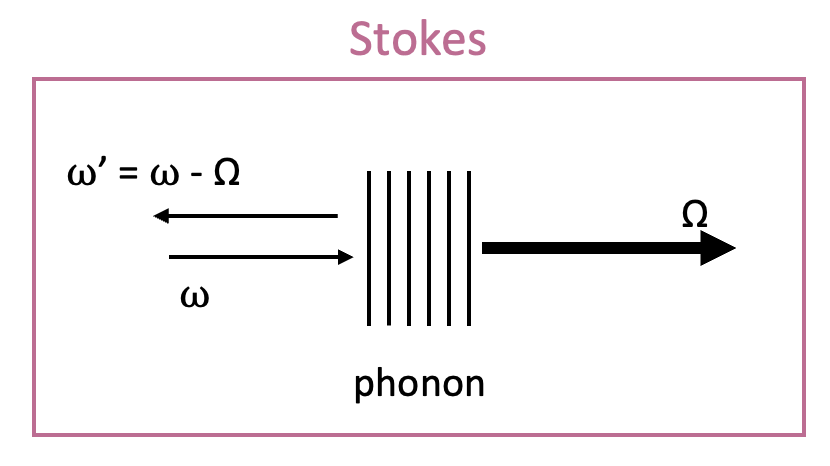
\includegraphics[width=\textwidth]{figs/2-Cooling/StokesHeatingProcess.png}
        \caption{}
        \label{fig:Cooling:StokesHeating}
    \end{subfigure}
    \hfill
    \begin{subfigure}[b]{0.49\textwidth}
        \centering
        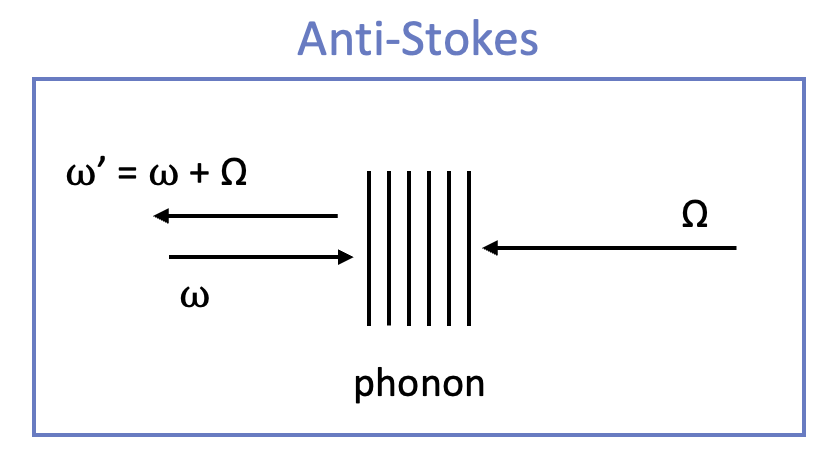
\includegraphics[width=\textwidth]{figs/2-Cooling/anti-StokesCoolingProcess.png}
        \caption{}
        \label{fig:Cooling:anti-StokesCooling}
    \end{subfigure}
    \caption[Illustration of optomechanical heating and cooling processes.]{Illustration of optomechanical heating and cooling processes. Figure \ref{fig:Cooling:StokesHeating} shows an incident photon of frequency \(\omega\) scattering with a retreating phonon of frequency \(\Omega\), resulting in the annihilation of the incident photon and the creation of both an additional retreating phonon of frequency \(\Omega\) and a backwards propagating photon down-shifted in frequency (\(\omega_{\rm Stokes} = \omega - \Omega\)). Figure \ref{fig:Cooling:anti-StokesCooling} shows the inverse process, whereby an incident photon, \(\omega\), scatters with an approaching phonon, \(\Omega\), annihilating the incident photon and the phonon to produce a backwards propagating photon up-shifted in frequency (\(\omega_{\mathrm{anti-Stokes}} = \omega + \Omega\)).}
    \label{fig:Cooling:StokesProcesses}
\end{figure}

\subsection{Spectral Signatures of Cooling and Heating}
\label{Cooling:subsec:SpectralSignaturesofCoolingandHeating}

Optomechanical cooling reduces the phonon occupation of a given mechanical mode. Evidence of this phenomenon is offered by changes in two key spectral features of the backscattered light: linewidth and amplitude. Spectral linewidth is a measure of the mechanical dissipation rate of the phonon mode. A broader linewidth corresponds with a faster mechanical dissipation rate of a given mode as per the time-energy uncertainty principle: greater dissipation means shorter phonon lifetime, which introduces an uncertainty in the phonon frequency. Thereby, increasing the dissipation rate (cooling) broadens the spectral linewidth; conversely, decreasing the dissipation rate (heating) narrows the spectral linewidth. For spontaneous Brillouin scattering this is given by \cite{otterstrom2018optomechanical}

\begin{equation}
  \Gamma_{\pm} \approx \Gamma_{0}\left(1 \pm \frac{G}{4}\right),
  \label{eq:Cooling:effective linewidth}
\end{equation}
\\
where \(\Gamma_{0}\) is the mechanical dissipation rate at thermal equilibrium, \(\Gamma_{\pm}\) is the effectively broadened (\(+\)) or narrowed (\(-\)) dissipation rate due to an anti-Stokes or Stokes process, respectively. Here, \(G\) is the Brilouin scattering process gain factor \(G = G_{\mathrm{B}}P_{\rm P}L\), where \(G_{\rm B}\) is the effective Brillouin gain (\si{\per\watt\per\meter}), \(P_{\rm P}\) is the pump power, and \(L\) is the effective length (see Section~\ref{appendix:comparison} in Appendix~\ref{appendix: CoBS}). Equation~\ref{eq:Cooling:effective linewidth} is related to the effective temperature change of the mechanical mode via the quantized phonon dissipation rate (phonons dissipated per second) at equilibrium, given by

\begin{equation}
  Q = n_{\rm th}\Gamma_{0},
  \label{eq:Cooling:Q}
\end{equation}
\\
where \(\Gamma_{0}\) is the mechanical dissipation rate at thermal equilibrium and \(n_{\rm th}\) is the mean thermal occupancy (phonon count) of the mode at equilibrium given by the Bose-Einstein distribution, or the Planck distribution function for phonons, \cite{kittel1980thermal}

\begin{equation}
  n_{\rm th} = \frac{1}{e^\frac{\hbar\Omega_{\rm B}}{k_{\rm B}T_{0}} - 1}.
  \label{eq:Cooling:nth}
\end{equation}
\\
Here, \(\hbar = h/2\pi\) is the reduced Planck constant, \(\Omega_{\rm B}\) is the angular phonon frequency, \(k_{\rm B}\) is the Boltzmann constant, and \(T_{0}\) is equilibrium (room) temperature in kelvin. Laser cooling of the phonon mode increases the effective dissipation rate of the mode by offering a new escape channel by which phonons may exit the mode (converting to the optical domain). This altered dissipation rate gives the effective temperature via Equation~\ref{eq:Cooling:Q},

\begin{equation}
  n_{\rm eff}\Gamma_{\pm} \approx n_{\rm th}\Gamma_{0},
  \label{eq:Cooling:nGamma}
\end{equation}
\\
where \(n_{\rm eff}\) is the effective phonon mode occupancy of the cooled (\(+\), widened dissipation rate) or heated (\(-\), narrowed dissipation rate). For \si{\giga\hertz} phonon frequencies near room temperature, \(k_{\rm B}T \gg \hbar\Omega_{\rm B}\), allowing the first order approximation

\begin{equation}
  e^{\frac{\hbar\Omega_{\rm B}}{k_{\rm B}T}} \approx 1 + \frac{\hbar\Omega_{\rm B}}{k_{\rm B}T},
\end{equation}
\\
which gives, for Equation~\ref{eq:Cooling:nth},

\begin{equation}
  n_{\rm th} \approx \frac{k_{\rm B}T_{0}}{\hbar\Omega_{\rm B}}.
\end{equation}
\\
Inserting this approximation in Equation~\ref{eq:Cooling:nGamma}, and in combination with Equation~\ref{eq:Cooling:effective linewidth}, we find two independent approximations for the ratio of effective to equilibrium temperatures of the cooled phonon mode,

\begin{equation}
  \frac{\Gamma_{+}}{\Gamma_{0}} \approx \frac{T_{0}}{T_{\rm eff}} \approx 1 + \frac{G}{4}.
\end{equation}
\\
Rearanging for fractional degrees cooled (\(\Delta T/T_{0}\)), where \(\Delta T = T_{0} - T_{\rm eff}\) is degrees cooled from equilibrium, we find (to first order approximation)

\begin{equation}
  \frac{\Gamma_{+}}{\Gamma_{0}} - 1 \approx \frac{\Delta T}{T_{0}} \approx \frac{G}{G + 4}.
  \label{eq:Cooliong:two methods of getting temperature}
\end{equation}

Spectral amplitude provides additional evidence of optomechanical cooling. Spectral amplitude is a measure of the scattered power produced from pump light scattering with phonons occupying a given mechanical mode. Higher phonon occupancy within a given mode provides a higher rate of scattering and thus a higher measured spectral amplitude of the backscattered light. Increasing pump power reduces the phonon population occupying the anti-Stokes mode and thereby lessens the otherwise scattered power, measured as spectral amplitude. The inverse process occurs for the Stokes process; increasing pump power increases the phonon population occupying the Stokes mode and thereby increases the otherwise scattered power, measured from spectral amplitude.

In the spontaneous Brillouin scattering process, however, scattered power increases not only with phonon population (linked to temperature via Equation~\ref{eq:Cooling:nth}), but also with pump power \(P_{\rm P}\) (see Equation~\ref{eq:sponBSscatteredPower} in Appendix~\ref{appendix:comparison}). As a result, both the Stokes and anti-Stokes spectral amplitudes increase with increasing pump power. Despite this, however, spectral amplitudes still provide evidence of laser cooling. Asymmetric growth rates of the relative Stokes and anti-Stokes spectral amplitudes with increasing pump power indicate underlying cooling of the anti-Stokes phonon mode relative to the Stokes. The anti-Stokes scattering process (phonon annihilation) leads to a sublinear growth trend in peak spectral amplitude even as increasing pump power raises the overall peak amplitude. Conversely, the Stokes scattering process (phonon creating) leads to a superlinear growth trend in peak spectral amplitudes as pump power raises. These divergent trends in peak spectral amplitudes are a direct result of the optomechanically-induced altering of the thermal state of the respective modes and provide key evidence of laser cooling.

To expand on this, one might imagine a process whereby a pump laser cools a medium through the anti-Stokes process while an independent probe laser is simultaneously co-injected and allowed to scatter with the same phonon mode being cooled by the pump. In this pump-probe arrangement, increasing pump power induces further cooling of the anti-Stokes mode just as before, but with the addition of a probe that may be held at constant power. Critically, while backscattered \emph{pump} light would still feature an overall growth trend in peak spectral amplitude (proportional to pump power), scattered power of the \emph{probe} would only be sensitive to the underlying phonon occupancy (temperature) of the mode. As such, for the anti-Stokes (cooling) process, peak amplitudes of the probe spectra would actually be seen to \emph{decrease} with increasing pump power, commensurate with the mode being increasingly cooled by the pump. As such, this pump-probe spectroscopy regime offers a direct measure of phonon occupancy, and thus direct and independent confirmation of laser cooling occurring.

\section{Methods}
\label{Cooling:sec:Methods}

While spontaneous Brillouin scattering processes naturally alter phonon populations (and thus mode temperatures), practical demonstration and detection of these effects pose significant challenges. Foremost among these is the requirement to remain in the spontaneous regime: we wish to probe the natural thermal phonons in a medium, so we cannot rely on artificially driving the mechanical modes to enhance scattered power (see Appendix~\ref{appendix:comparison}, and specifically Figure~\ref{fig:SponBSvsStimBSvsCoBS}, for a comparison of scattered power produced by different Brillouin techniques). Although stimulated Brillouin scattering (SBS) is often employed to boost signal levels, it actively drives phonon populations via injected optical fields, and thus no longer measures the intrinsic thermal phonons. In practical terms, SBS occurs when the overall process gain factor \(G = G_{\rm B}P_{\rm P}L\) (where \(G_{\rm B}\) is the effective Brillouin gain, \(P_{\rm P}\) the pump power, and \(L\) the effective length) far exceeds unity (\(G \gg 1\)).

To demonstrate optomechanical cooling (i.e., an anti-Stokes process that lowers phonon energy), one must detect scattered light from a mode whose phonon population has been reduced. This is intrinsically difficult because a decreased phonon population means fewer scattering events, and hence diminished backscattered light. Consequently, an ideal testbed should provide sufficiently high single-pass gain (overall gain factor near unity) to enable clear detection, yet remain below the threshold that would drive the process into the stimulated regime. Although the Stokes and anti-Stokes processes address distinct phonon modes in a traveling-wave system, allowing any mode to become stimulated generates large driven phonon populations that can obscure or counteract spontaneous cooling. Achieving this balance ensures that measurements reflect genuine spontaneous cooling of a thermally populated phonon mode, rather than an artifact of optically driven phonons.

In addition to the requirement that the overall process gain be near but below unity, temporal constraints impose further critical conditions. Specifically, the rate at which phonons are removed from the system must exceed the rate at which they are replenished by the thermal bath to ensure net cooling of the anti-Stokes mode. This condition demands that backscattered photons leave the system rapidly, carrying away the extracted mechanical energy. A mean-field analysis (see Appendix~A of Johnson et al. 2023 \cite{johnson2023laser}) shows that the relevant depletion rate is \(4v_{\rm g}/L\), where \(v_{\rm g}\) is the group velocity of the anti-Stokes light and \(L\) is the system length. This must exceed the mechanical dissipation rate \(\Gamma_{\rm 0}\), which represents the natural return of the phonon mode to thermal equilibrium. Hence, a suitable platform for demonstrating optomechanical cooling of traveling-wave phonons must fulfill the fast escape condition \(4v_{\rm g}/L > \Gamma_{\rm 0}\). Meeting this requirement on system length, however, directly conflicts with the desire for a sufficiently high overall gain factor, illustrating the delicate balance needed for effective cooling.

%--------------------------------------------------------------------%

\subsection{\texorpdfstring{\ce{CS2}}{CS2}-Filled Liquid-Core Optical Fiber}
\label{Cooling:subsec:CS2FilledLCOF}

\begin{figure}[t]
  \centering
  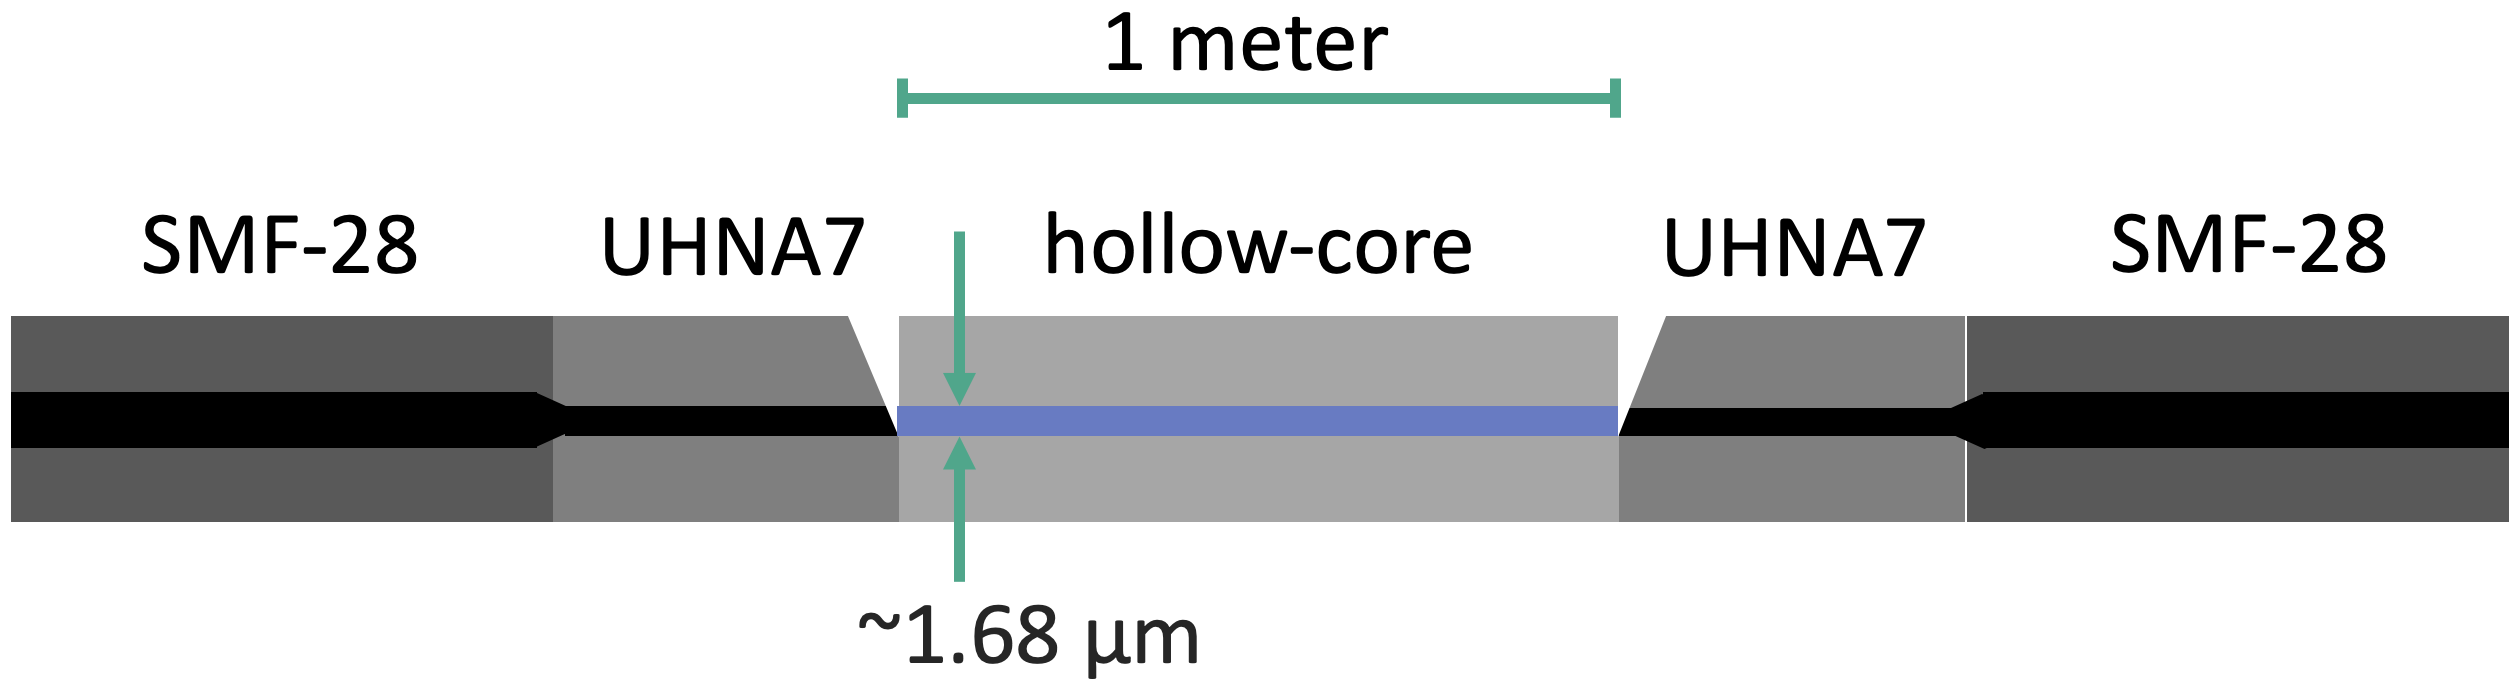
\includegraphics[width=\textwidth]{figs/2-Cooling/LCOFdiagram.png}
  \caption[Schematic of \ac{LCOF} design.]{Schematic of \ac{LCOF} design. A length of \ac{SMF-28} is arc-spliced to 5-\SI{10}{\centi\meter} of \ac{UHNA7} fiber, with a post-arc process applied to taper the larger \ac{SMF-28} core down to the smaller \ac{UHNA7} core for better mode matching and coupling efficiency. The \ac{UHNA7} fiber is angle-cleaved and fusion-spliced to a flat-cleaved hollow-core fiber via a heated filament in a Vytran fusion splicer system. The angle cleave results in a splice that only partially fuses the two fibers, leaving a pathway for liquid to enter the hollow core fiber via capillary action once submerged. A mirrored splice configuration on the other end of the length of hollow-core fiber allows air to escape as the fiber fills, and a reverse taper again provides improved mode matching for the light to recouple into \ac{SMF-28}.}
  \label{fig:LCOF diagram}
\end{figure}

To demonstrate optomechanical cooling of traveling wave phonons, we utilize \SI{1}{\meter} of \acl{LCOF} filled with carbon disulfide, first developed by Kieu et al. (2012). \cite{kieu2012integrated} This platform features large optomechanical coupling due to the high electrostritive response of \ce{CS2} \cite{boyd2020nonlinear} and the small effective area defining acousto-optic mode overlap offered by the small \SI{0.9}{\micro\meter} core radius of the capillary fiber. These characteristics of the \ac{LCOF} system combine to produce an effective Brillouin gain coefficient \(G_{\rm B} >\)~\SI{2}{\per\watt\per\meter}, enabling sufficient scattering within the relatively short length required to satisfy the fast-escape condition \(4v_{\rm g}/L > \Gamma_{0}\) (\(4v_{\rm g}/L \approx\) \SI{0.82}{\giga\hertz} and \(\Gamma_{0} \approx\) 2\(\pi\times\)\SI{97}{\mega\hertz} \(\approx\) \SI{0.61}{\giga\hertz}). \cite{johnson2023laser} Additionally, this \ce{CS2}-filled \ac{LCOF} system provides excellent acoustic and optical guidance due to the large electromagnetic and acoustic impedance differential between the \ce{CS2} core and surrounding silica. \cite{behunin2019spontaneous}

Figure~\ref{fig:LCOF diagram} shows a schematic of the \ac{LCOF} design. Coupling into and out of the \ac{LCOF} is facilitated by a short length of tapered \ac{UHNA7} for better mode matching between the \SI{4.8}{\micro\meter} core radius \ac{SMF-28} and the \SI{0.84}{\micro\meter} core radius of the capillary fiber. An angled cleave of the \ac{UHNA7} fiber allows for a small wedge gap to remain after fusion splicing to the capillary fiber. This gap allows liquid \ce{CS2} to enter and fill the hollow core of the fiber via capillary action. Appendix~\ref{Cooling:Appendix:sec:FabricationofCS2FilledLCOF} describes the fabrication and filling processes of the \ac{LCOF} and details key insights which contributed to significant reductions in failure rate as well as time and material cost of sample preparation.

%--------------------------------------------------------------------%

\subsection{Cooling Experiment~A: Spontaneous Brillouin Cooling}
\label{Cooling:subsec:ExperimentASpontaneousBrillouinCooling}

We conducted two independent experiments to demonstrate and verify laser cooling of traveling wave phonons in our \ce{CS2}-\ac{LCOF} platform. The first experiment (Experiment~A) employs a pump laser to launch \SI{1.55}{\micro\meter} light into the \ac{LCOF}. The backscattered Stokes and anti-Stokes components are filtered and collected by a detector. In this experiment, evidence of cooling is given by symmetry breaking between the amplitudes and widths of the Stokes and anti-Stokes spectra as pump power is varied. Backscattered pump light is shifted in frequency by a band of frequencies centered at the resonant Brillouin frequency of the \ac{LCOF} (\(\Omega_{\rm B,\,LCOF} \approx 2\pi\times\SI{2.27}{\giga\hertz}\)).

These backscattered signals exhibit a spectral linewidth corresponding to the mechanical dissipation rate in the phonon mode (conversely, finite phonon lifetime). The polarization state of the backscattered pump and probe light is recovered after retracing their paths, permitting only probe light to transmit through the \ac{PBS} for filtration and heterodyne detection. Output from the detector is again amplified by an \ac{RF} amplifier and routed to an \ac{RFSA} for data collection. With the probe power inside the \ac{LCOF} held constant, changes in the amplitude and width of the probe spectra provide direct evidence of laser cooling from varying pump powers within the \ac{LCOF}.

Figure~\ref{fig:Cooling:ExperimentADesign} shows a schematic diagram of the experimental setup for Experiment~A. A \ac{CW} pump laser emitting at \SI{1.55}{\micro\meter} (\(\omega_{\rm P}\)) is amplified by an \ac{EDFA} and its power is controlled by a \ac{VOA}. This light is subsequently routed via a circulator to the \ce{CS2}-\ac{LCOF}, where some of the light backscatters within the length of the \ac{LCOF}. Backscattered light is frequency-shifted, up for anti-Stokes (\(\omega_{\rm aS} = \omega_{\rm P} + \Omega_{\mathrm{B}}\)) and down for Stokes
(\(\omega_{\rm S} = \omega_{\rm P} - \Omega_{\rm B}\)),
by a band of frequencies centered around the Brillouin frequency of the \ac{LCOF} (\(\Omega_{\rm B,\,LCOF} \approx\) \SI{2.27}{\giga\hertz}). Backscattered light is routed by circulators to a \SI{5}{\giga\hertz} \ac{BPF} to allow selection of either the Stokes or anti-Stokes light while also reducing unwanted frequency noise. The filtered signal is then incident on a photodiode detector sensitive to \si{\giga\hertz} frequencies. A \ac{LO} is synthesized from the pump laser, polarization controlled, amplified, and combined with the signal pre-detector for heterodyne detection. Output from the detector is amplified with a \ac{RF} amplifier and sent to a \ac{RFSA} for data collection.

To conduct the experiment, pump power was varied from \SI{10}{\milli\watt} to \SI{290}{\milli\watt} in increments of \SI{10}{\milli\watt}, as measured pre-injection into the \ac{LCOF}, and respective Stokes and anti-Stokes spectra for each pump power were collected sequentially by tuning the placement of the \ac{BPF}. For both the Stokes and anti-Stokes modes, five repeated measurements of each spectra and the background (pump off) were collected for each pump power, with each measurement comprising an average over 100 \SI{250}{\milli\second} sweeps at a \ac{RBW} of \SI{1}{\mega\hertz}. Optical transmission through the entire \ac{LCOF} sample which was used for the published data was measured to be 17\%, giving \(100\sqrt{0.17} \approx 41\%\) transmission through just the first splice assuming equal transmission through both \ac{LCOF} splices. This provided a scaling factor for obtaining intrafiber powers from injected pump power (\(P_{\rm intrafiber} = \sqrt{0.17}P_{\rm P}\)) which was used for data processing and analysis for the publication.

\begin{figure}[t]
  \centering
  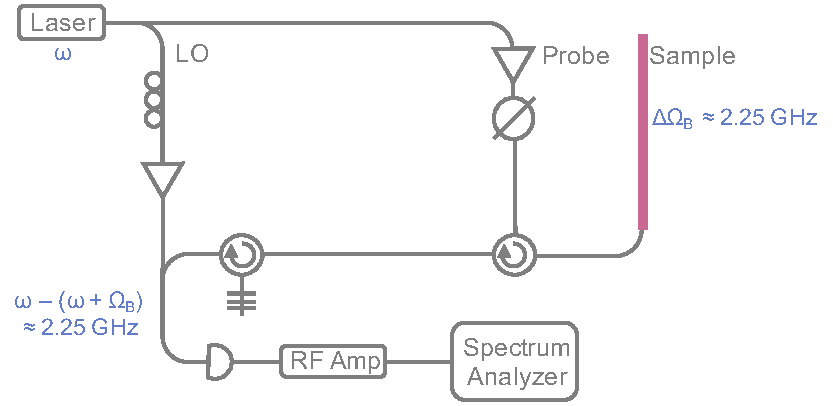
\includegraphics[width=\textwidth]{figs/2-Cooling/pumpOnlyDesign.pdf}
  \caption[Schematic of experimental setup for Experiment~A.]{Schematic of experimental setup for Experiment~A. In this experiment, a \ac{CW} pump laser emitting at \SI{1.55}{\micro\meter} is amplified, passed through a circulator, and injected into the \ce{CS2}-\ac{LCOF}. Backscattered light is routed to a \ac{BPF} for selection of Stokes or anti-Stokes frequencies and sent to a detector. A \ac{LO} is synthesized from the pump laser for heterodyne detection, whereby a \acl{PC} is used to align the polarization of the \ac{LO} to that of the backscattered signal. The signal passes through a \acl{RF} amplifier before being sent to a \ac{RFSA} for collection. Pump power is controlled by a \ac{VOA} placed just after the \ac{EDFA}. Stokes and anti-Stokes spectra are collected sequentially for each pump power by adjusting the placement of the \ac{BPF}.}
  \label{fig:Cooling:ExperimentADesign}
\end{figure}

\subsection{Cooling Experiment~B: Pump-Probe Verification}
\label{Cooling:subsec:ExperimentBPump-ProbeVerification}

A second experiment (Experiment~B) was conducted to provide direct evidence of cooling via pump-probe spectroscopy, whereby a separate probe laser is held at constant power while a pump laser is varied to affect cooling in the \ac{LCOF}. In Experiment~B, backscattered light from the probe laser provides direct evidence of cooling through spectral changes in amplitude and linewidth as pump power is independently varied. To achieve independence of the pump and probe, probe light was controlled to be polarized orthogonal to the pump.

Figure~\ref{fig:Cooling:ExperimentBDesign} shows a schematic of the experimental design for Experiment~B. Starting from a single \ac{CW} laser operating at \SI{1.55}{\micro\meter}, we generate a pump \(\omega_{\rm P}\), probe \(\omega_{\rm Pr}\), and \ac{LO}. A \ac{PBS} combines the pump and probe for co-injection into the \ac{LCOF}. The pump light is amplified by an \ac{EDFA}, and its polarization is adjusted so that it reflects at the \ac{PBS} for launching into the \ac{LCOF}. The probe light passes through a circulator and is polarization-adjusted to transmit through the \ac{PBS} for injection into the \ac{LCOF}. A 99-1 splitter directs 1\% of the combined pump and probe light to a second \ac{PBS} for monitoring of respective powers injected into the \ac{LCOF}.

\begin{figure}[t]
  \centering
  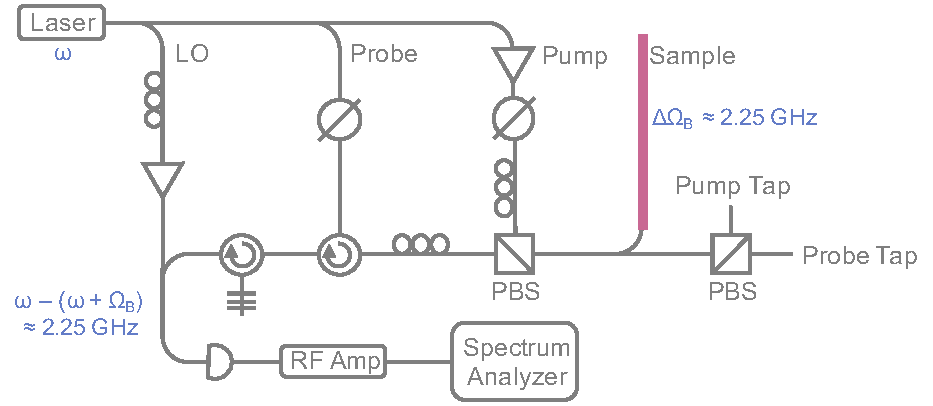
\includegraphics[width=\textwidth]{figs/2-Cooling/pumpProbeDesign.pdf}
  \caption[Schematic of experimental setup for Experiment~B.]{Schematic of experimental setup for Experiment~B. A pump, probe, and \ac{LO} are generated from a single \ac{CW} laser operating at \SI{1.55}{\micro\meter}. Pump light is amplified and directed through a \ac{VOA} and \ac{PC}, where its polarization is adjusted to reflect at the \ac{PBS}. Probe light passes through a \ac{VOA} for careful power control across measurement sets before being routed by a circulator to the \ac{PBS}. Polarization of the probe light is adjusted for transmission through the \ac{PBS} for co-injection with the pump into the \ac{LCOF}. A 99-1 splitter directs 1\% of the total pump and probe light to a second \ac{PBS} for monitoring of respective powers injected injected into the \ac{LCOF}. Backscattered Stokes and anti-Stokes components of both the pump and the probe retrace to the first \ac{PBS}, where the respective polarization states of each ensure a re-separation of backscattered pump and probe light. The probe light is filtered by a tunable \ac{BPF} and heterodyned with the \ac{LO} prior to detection. Detector output is amplified by an \ac{RF} amplifier and fed to an \ac{RFSA} for data collection.}
  \label{fig:Cooling:ExperimentBDesign}
\end{figure}

Backscattered light from both the pump and the probe is shifted in frequency by approximately the Brillouin frequency of the \ac{LCOF} (\(\Omega_{\rm B,\,LCOF} \approx \SI{2.27}{\giga\hertz}\)). The frequencies and wavevectors involved in both the pump and the probe scattering processes satisfy similar phase matching conditions given by Equation~\ref{eq:Cooling:anti-Stokes Phase Matching}. Because this pump-probe technique provides a direct measure of laser cooling, only the anti-Stokes spectra need to be collected. In conducting the experiment, five repeated measurements of both the anti-Stokes spectra and the background (pump off) were collected for each pump power, with each measurement comprising an average over 100 \SI{250}{\milli\second} sweeps at a \ac{RBW} of \SI{1}{\mega\hertz}.

Notably, this experiment relies on careful control of the polarization states of the pump and the probe. Upon backscattering within the \ac{LCOF}, their respective polarization states are recovered after retracing their paths to the \ac{PBS}, which ensures only probe light transmits through the \ac{PBS} for filtration and heterodyne detection. Output from the detector is amplified by an \ac{RF} amplifier and routed to an \ac{RFSA} for data collection. In this way, by holding the probe power inside the \ac{LCOF} constant, changes in the amplitude and width of the backscattered probe spectra provide direct and independent evidence of laser cooling from varying pump powers within the \ac{LCOF}.

%--------------------------------------------------------------------%

\section{Results}
\label{Cooling:sec:Results}


\subsection{Cooling Experiment~A Results}
\label{Cooling:subsec:ExperimentAResults}

Figures~\ref{fig:Cooling:P-O Stokes} and \ref{fig:Cooling:P-O anti-Stokes} show the respective Stokes and anti-Stokes spectra gathered across a range of intra-fiber pump powers, from \SI{4.12}{\milli\watt} to \SI{119.57}{\milli\watt}. Both Stokes and anti-Stokes spectra sets are centered at approximately \(f_{\rm B} = \) \SI{2.27}{\giga\hertz}, representing the respective up- and downshift from the pump frequency by the Brillouin frequency of the \ce{CS2}-\ac{LCOF} at \SI{1.55}{\micro\meter}. For increasing pump power, we see an asymmetry in evolution of peak spectral densities and of the Stokes and anti-Stokes spectra, a key fingerprint of optomechanical cooling. Figure~\ref{fig:Cooling:P-O Heights vs Pow} plots the lorentzian-fitted Stokes and anti-Stokes peak amplitudes for each pump power. A dashed line showing a linear trend was obtained by applying a linear fit of all data points. Solid lines show the theoretical super- and sublinear scattered power for the Stokes and anti-Stokes processes, respectively, and were calculated using Equations~A27 and A28 in Appendix~A of Johnson et al. (2023)\cite{johnson2023laser}. Figure~\ref{fig:Cooling:P-O Heights vs Pow} shows that peak amplitudes of both processes are in good alignment of the theoretical trend, with anti-Stokes peaks increasing sublinearly and Stokes peaks increasing superlinearly.

This is consistent with one of the key signatures of laser cooling: as higher pump powers further reduce the phonon occupation within the anti-Stokes mode (cooling), scattered power falls farther short of the otherwise linear relationship with pump power (Equation~\ref{eq:sponBSscatteredPower}). This sublinear trend in scattered power produces the same trend in backscattered light incident on the detector and reveals itself in the data as a sublinear trend in peak spectral density with increasing pump power. The opposite effect occurs in the Stokes process; as higher pump powers further increase the phonon occupation within the Stokes mode (heating), scattered power rises further above the otherwise linear relationship with pump power (again given by Equation~\ref{eq:sponBSscatteredPower}). This superlinear trend in scattered power produces the same trend in backscattered light incident on the detector and reveals itself in the data as a superlinear trend in peak spectral density with increasing pump power. These respective super- and sublinear growth trends in peak amplitudes of the Stokes and anti-Stokes spectra as pump power increases provide a spectral fingerprint of optomechanical cooling of the anti-Stokes phonon mode within the \ac{LCOF}.

\begin{figure}[t!]
  \centering
  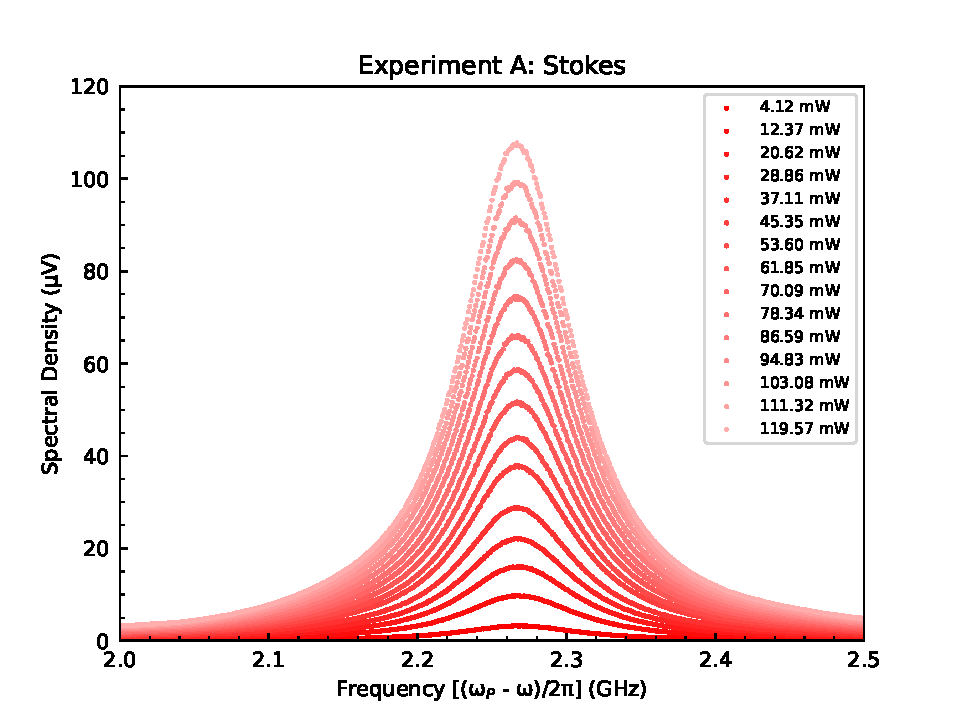
\includegraphics[width=\textwidth]{figs/2-Cooling/P-O Stokes.pdf}
  \caption[Stokes spectra for a range of pump powers obtained for Experiment~A via spontaneous backwards Brillouin scattering.]{Stokes spectra for a range of pump powers obtained for Experiment~A via spontaneous backwards Brillouin scattering. Intrafiber pump powers are displayed and were calculated from a measurement of 17\% total through-fiber transmission and assuming equal losses through each of the two splices bookending the \ac{LCOF}. To obtain each spectra, five repeated measurements of both the Stokes spectra and the background (pump off) were collected for each pump power, with each measurement comprising an average over 100 \SI{250}{\milli\second} sweeps at a \ac{RBW} of \SI{1}{\mega\hertz}. Plotted are the resulting background-subtracted spectra, with uncertainties smaller than the data point markers.}
  \label{fig:Cooling:P-O Stokes}
\end{figure}

\begin{figure}[t!]
  \centering
  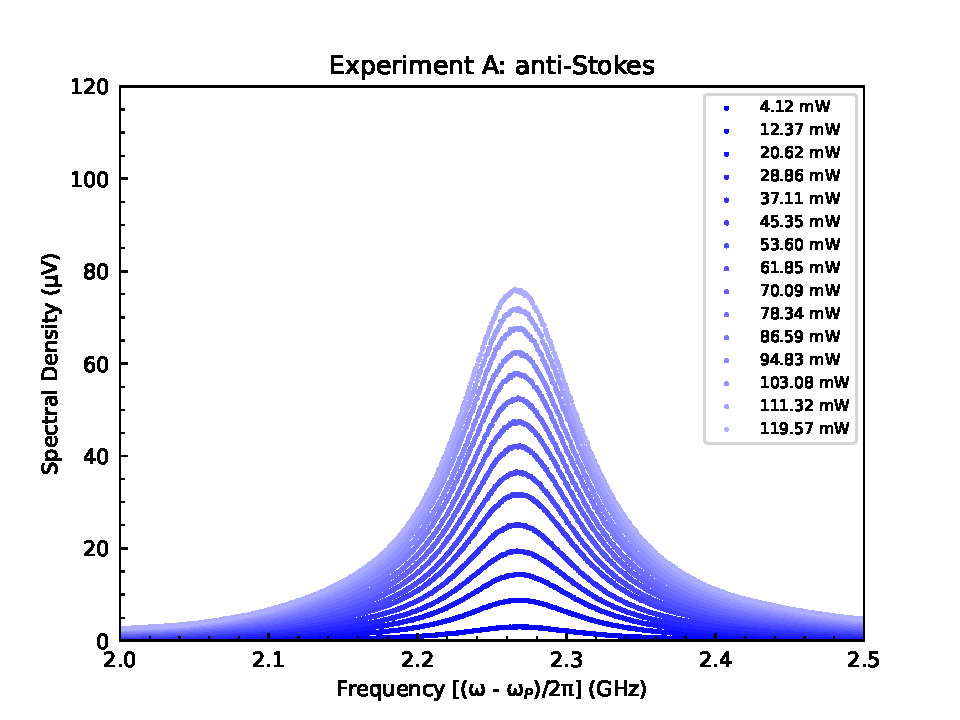
\includegraphics[width=\textwidth]{figs/2-Cooling/P-O anti-Stokes.pdf}
  \caption[Anti-Stokes spectra for a range of pump powers obtained for Experiment~A via spontaneous backwards Brillouin scattering.]{Anti-Stokes spectra for a range of pump powers obtained for Experiment~A via spontaneous backwards Brillouin scattering. Intrafiber pump powers are displayed and were calculated from a measurement of 17\% total through-fiber transmission and assuming equal losses through each of the two splices bookending the \ac{LCOF}. To obtain each spectra, five repeated measurements of both the anti-Stokes spectra and the background (pump off) were collected for each pump power, with each measurement comprising an average over 100 \SI{250}{\milli\second} sweeps at a \ac{RBW} of \SI{1}{\mega\hertz}. Plotted are the resulting background-subtracted spectra, with uncertainties smaller than the data point markers.}
  \label{fig:Cooling:P-O anti-Stokes}
\end{figure}

Linewidths of the spectra shown in Figures~\ref{fig:Cooling:P-O Stokes} and \ref{fig:Cooling:P-O anti-Stokes} also exhibit key spectral signatures of laser cooling (and heating for the Stokes mode). With increasing pump power, the linewidths of the anti-Stokes spectra broaden, indicating a higher dissipation rate of phonons into the “optical bath” (cooling). The inverse trend is seen for the Stokes mode: with increasing pump power, the linewidths of the Stokes spectra narrow, indicating a reduced phonon dissipation rate (heating). Figure~\ref{fig:Cooling:P-O Linewidths} plots the Stokes and anti-Stokes linewidths for each pump power, obtained from a lorentzian fit. Solid lines provide a linear fit to the respective Stokes and anti-Stokes measured linewidths. The secondary y-axis provides a temperature scale in degrees \si{\kelvin}, with room temperature (taken to be \SI{293}{\kelvin}) centered at the equilibrium linewidth of the \ac{LCOF}. Section~\ref{Cooling:Appendix:subsec:Experiment A Tabulated Values} provides a tabulation of the extracted fit parameters and their associated uncertainties for each of the Stokes and anti-Stokes spectra for all pump powers.

Using Equation~\ref{eq:Cooling:effective linewidth} and the respective broadened and equilibrium anti-Stokes linewidths at the highest intrafiber pump power (\(\Gamma_{\text{\(P_{\rm P} = \SI{119.57}{\milli\watt}\)}} = \SI{106.32}{\mega\hertz}\)) as compared to the lowest (\(\Gamma_{\text{\(P_{\rm P} = \SI{4.12}{\milli\watt}\)}} = \SI{97.3}{\mega\hertz}\)), we find an effective Brillouin gain \(G_{\rm B} \approx \SI{3.1(0.5)}{\per\watt\per\meter}\). Using this gain factor, we find  (right side of Equation~\ref{eq:Cooliong:two methods of getting temperature}) the temperature of the band of traveling wave phonons in the \ac{LCOF} to reduced by \(\Delta T \approx \SI{25(2)}{\kelvin}\) from room temperature. Using instead the phonon occupancy method (left side of Equation~\ref{eq:Cooliong:two methods of getting temperature}) with the same respective linewidths, we find \(\Delta T \approx \SI{27(2)}{\kelvin}\), which agrees with the prior calculation and is independent of estimated Brillouin gain and intrafiber pump powers. All measured values and their associated uncertaintites are tabulated for reproducability in Tables~\ref{tab:Cooling:Experiment A anti-Stokes} and \ref{tab:Cooling:Experiment A Stokes} in Appendix~\ref{Cooling:Appendix}, Section~\ref{Cooling:Appendix:sec:Tabulated Fit and Uncertainty Values Derived From the Experimental Data}. The published article associated with this work reports a conservatively calculated Brillouin gain of \SI{2.3}{\per\watt\per\meter}, also obtained from measured linewidths and Equation~\ref{eq:Cooling:effective linewidth}. This discrepency arises from slight differences in measured linewidths of the anti-Stokes spectra, which we attribute to variations among weighted fitting algorithms and resulting uncertainties. Using this reported value of \(G_{\rm B}\sim\)\SI{2.3}{\per\watt\per\meter} for the Brillouin gain along with the right side of Equation~\ref{eq:Cooliong:two methods of getting temperature} recovers the conservatively reported \(\sim\)\SI{21}{\kelvin} of cooling.

\begin{figure}[t!]
  \centering
  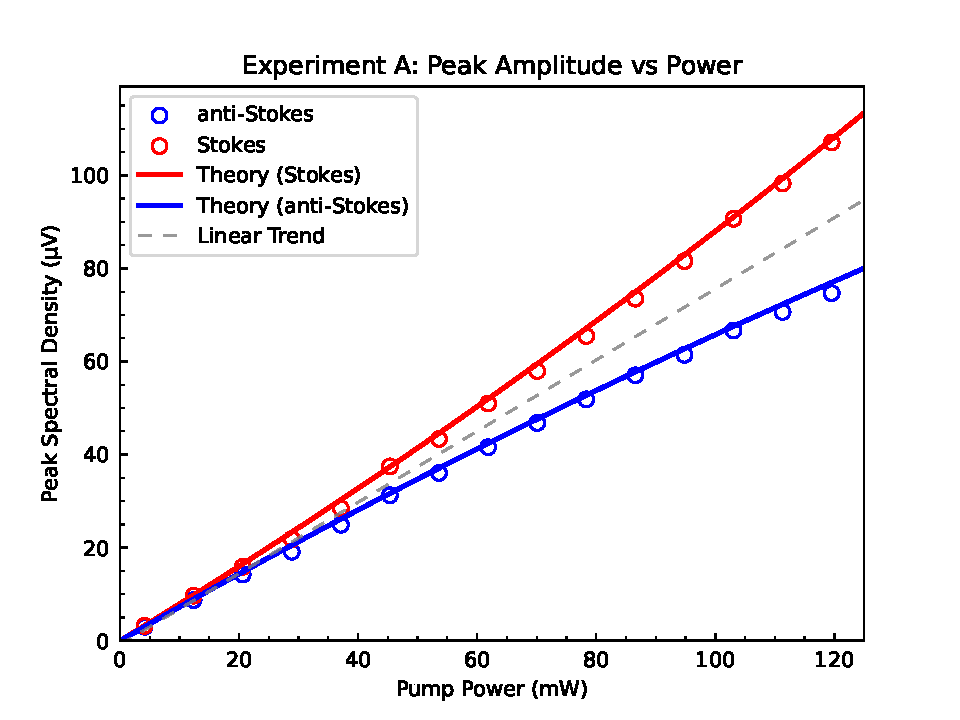
\includegraphics[width=\textwidth]{figs/2-Cooling/P-O Heights vs Pow.pdf}
  \caption[Lorentzian-fitted peak amplitudes of the observed Stokes and anti-Stokes spectra.]{Lorentzian-fitted peak amplitudes of the observed Stokes and anti-Stokes spectra. The dashed line showing a linear trend was obtained by applying a linear fit of all data points. The solid lines show the theoretical super- and sublinear scattered power for the Stokes and anti-Stokes processes, respectively, and were calculated using Equations~A27 and A28 in Appendix~A of Johnson et al. (2023) \cite{johnson2023laser}. Section~\ref{Cooling:Appendix:subsec:Experiment A Tabulated Values} provides a tabulation of the extracted fit parameters and their associated uncertainties for each of the Stokes and anti-Stokes spectra for all pump powers.}
  \label{fig:Cooling:P-O Heights vs Pow}
\end{figure}

\begin{figure}[t!]
  \centering
  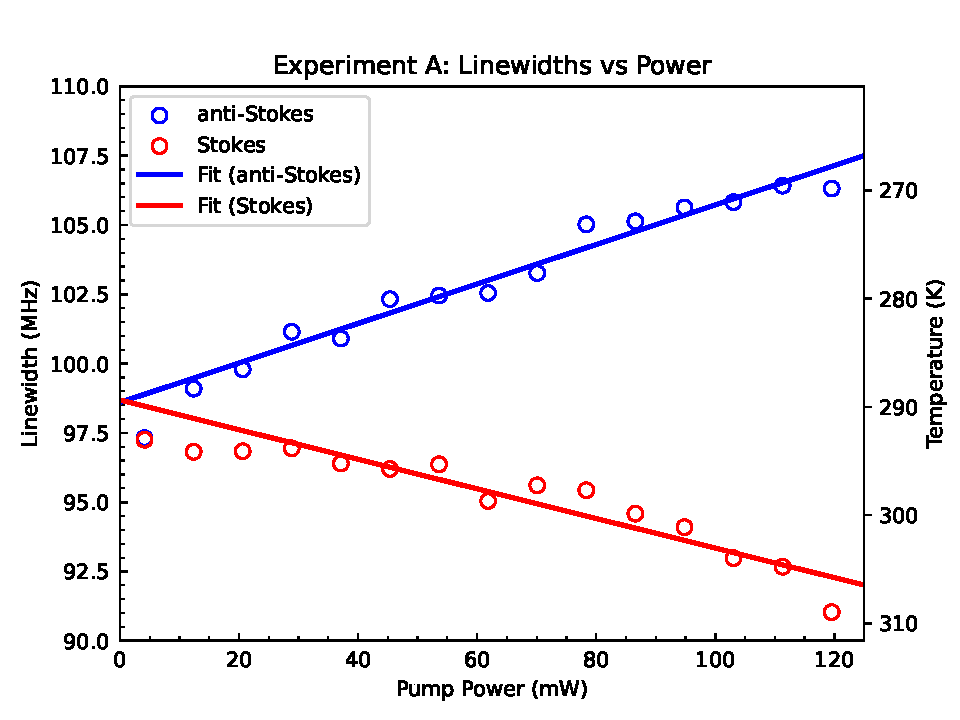
\includegraphics[width=\textwidth]{figs/2-Cooling/P-O Linewidths.pdf}
  \caption[Stokes and anti-Stokes linewidths for each pump power, obtained from a lorentzian fit.]{Stokes and anti-Stokes linewidths for each pump power, obtained from a lorentzian fit. Solid lines provide a linear fit to the respective Stokes and anti-Stokes measured linewidths. The secondary y-axis provides a temperature scale in degrees \si{\kelvin}, with room temperature (taken to be \SI{293}{\kelvin}) centered at the equilibrium linewidth of the \ac{LCOF}. Section~\ref{Cooling:Appendix:subsec:Experiment A Tabulated Values} provides a tabulation of the extracted fit parameters and their associated uncertainties for each of the Stokes and anti-Stokes spectra for all pump powers.}
  \label{fig:Cooling:P-O Linewidths}
\end{figure}

Figure~\ref{fig:Cooling:P-O Simulated Gain} plots a simulated Brillouin gain spectrum \(G_{\rm B}\) (\si{\per\watt\per\meter}), obtained from finite element simulations \cite{johnson2023laser} of the optical and acoustic modes of the \ac{LCOF}, overtop the \SI{4.12}{\milli\watt} pump power (nearest to natural equilibrium) anti-Stokes spectrum. While the y-scaling between the two spectra is arbitrary, the lorentzian profile of the gain spectrum, and specifically the center frequency and natural-equilibrium linewidth, is predictive of scattered power expected from the \ac{LCOF} across the frequency range. An uncertainty-weighted reduced \(\chi^{2}\) test for goodness of fit of the simulated gain spectrum to the observed anti-Stokes spectrum yields a value of 2.57. Reduced \(\chi^{2}\) values close to unity indicate a good fit.

\begin{figure}[t!]
  \centering
  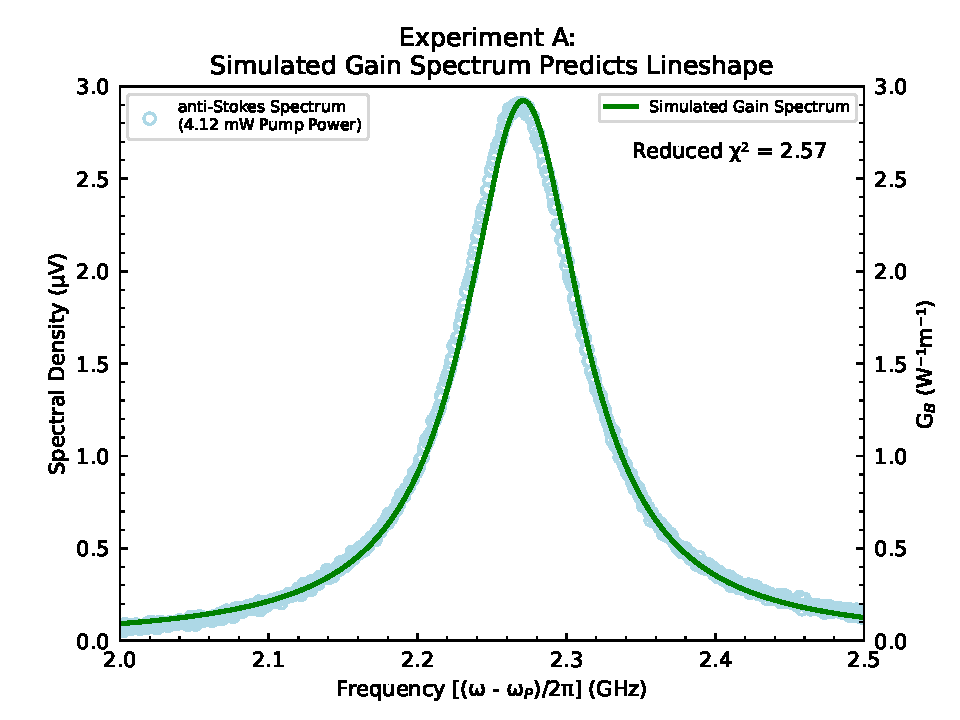
\includegraphics[width=\textwidth]{figs/2-Cooling/P-O Simulated Gain.pdf}
  \caption[A simulated Brillouin gain spectrum \(G_{\rm B}\) of the \ac{LCOF}, overtop the lowest power anti-Stokes spectrum.]{A simulated Brillouin gain spectrum \(G_{\rm B}\) (\si{\per\watt\per\meter}), obtained from finite element simulations \cite{johnson2023laser} of the optical and acoustic modes of the \ac{LCOF}, overtop the lowest power (nearest to natural equilibrium) anti-Stokes spectrum (the \SI{4.12}{\milli\watt} pump power spectrum). While the y-scaling between the two spectra is arbitrary, the lorentzian profile of the gain spectrum, and specifically the center frequency and natural-equilibrium linewidth, is predictive of scattered power expected from the \ac{LCOF} across the frequency range. An uncertainty-weighted reduced \(\chi^{2}\) test for goodness of fit of the simulated gain spectrum to the observed anti-Stokes spectrum yields a value of 2.57. Reduced \(\chi^{2}\) values close to unity indicate a good fit.}
  \label{fig:Cooling:P-O Simulated Gain}
\end{figure}


\subsection{Cooling Experiment~B Results}
\label{Cooling:subsec:ExperimentBResults}

Anti-Stokes scattered probe power was collected for four pump powers launched into the \ac{LCOF}, providing intrafiber pump powers of \SI{0.0}{\milli\watt}, \SI{22.7}{\milli\watt}, \SI{45.4}{\milli\watt}, and \SI{68.0}{\milli\watt}. Figures~\ref{fig:Cooling:P-P anti-Stokes Fit - 0mW}, \ref{fig:Cooling:P-P anti-Stokes Fit - 55mW}, \ref{fig:Cooling:P-P anti-Stokes Fit - 110mW}, and \ref{fig:Cooling:P-P anti-Stokes Fit - 165mW} show these resulting spectra, respectively, along with associated weighted Lorentzian fit for each. The data plotted data has been binned within \SI{10}{\mega\hertz} bins for clarity, with the Lorentzian fits and associated parameters having been derived from the unbinned data. Visual inspection confirms an excellent fit for each of the Lorentzian fits to their respective data, which have been plotted with error bars representing 1\(\sigma\) of the spectral density for each data point. All measured and calculated values are tabulated in Table~\ref{tab:Cooling:Experiment B} in Appendix~\ref{Cooling:Appendix}, Section~\ref{Cooling:Appendix:subsec:Experiment B Tabulated Values}, including solved fit parameters and their associated uncertainties.

\begin{figure}[t!]
  \centering
  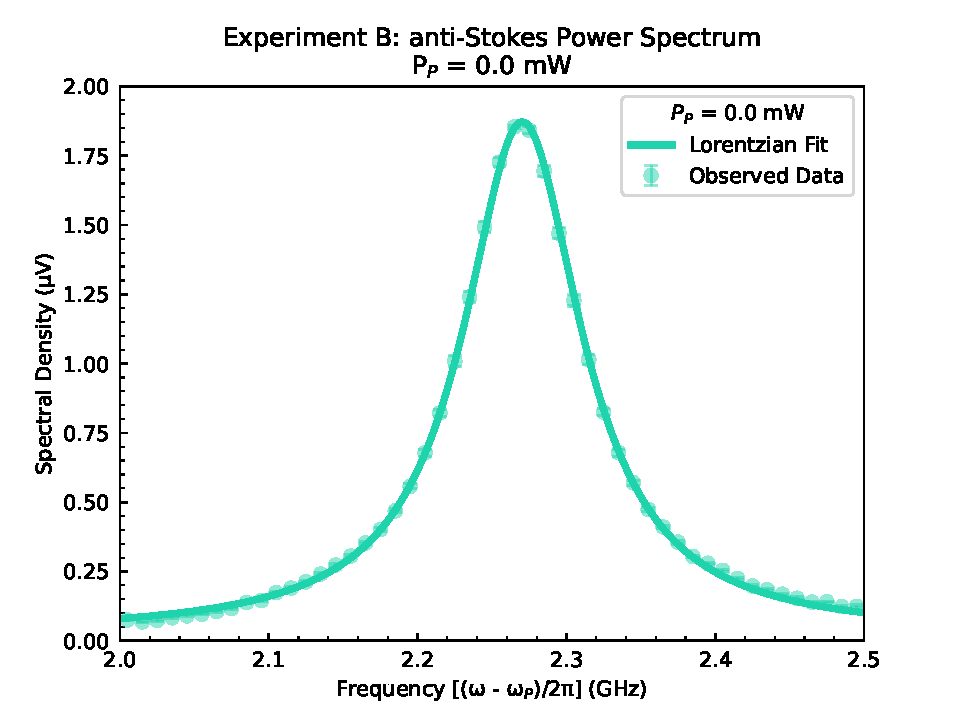
\includegraphics[width=\textwidth]{figs/2-Cooling/P-P anti-Stokes Fit - 0mW.pdf}
  \caption[Anti-Stokes probe spectra collected for \SI{0.0}{\milli\watt} intrafiber pump power in Experiment~B.]{Anti-Stokes probe spectra collected for \SI{0.0}{\milli\watt} intrafiber pump power in Experiment~B. Data is binned within \SI{10}{\mega\hertz} bins and displayed with error bars representing 1\(\sigma\) of spectral density. A Lorentzian fit has been computed based on the unbinned data and visual inspection confirms an excellent fit to the observed spectra. In conducting the experiment, five repeated measurements of both the anti-Stokes spectra and the background (pump off) were collected for each pump power, with each measurement comprising an average over 100 \SI{250}{\milli\second} sweeps at a \ac{RBW} of \SI{1}{\mega\hertz}. The spectral data shown here are the resulting background-subtracted spectra, with uncertainties propagated accordingly.}
  \label{fig:Cooling:P-P anti-Stokes Fit - 0mW}
\end{figure}

Figure~\ref{fig:Cooling:P-P anti-Stokes Fits} plots just the resulting fits for each spectra, showing a clear decrease in peak spectral amplitude with increasing pump power, consistent with the theory (see Equation~\ref{eq:sponBSscatteredPower} in Appendix~\ref{appendix:comparison}, with constant power yet decreasing modal temperature). Figure~\ref{fig:Cooling:P-P anti-Stokes Height v Pow} plots these peak spectral heights, derived from the fits, with their associated 1\(\sigma\) uncertainties. A linear fit has been applied, showing good correlation with the decreasing trend in peak spectral densities with increased pump power (cooling) corresponding to a lowering of the temperature of the anti-Stokes phonon mode. Figure~\ref{fig:Cooling:P-P anti-Stokes Wid v Pow} plots the spectral linewidths derived from the fits presented in Figure~\ref{fig:Cooling:P-P anti-Stokes Fits}, with their associated 1\(\sigma\) uncertainties. A linear fit has been applied, showing fair correlation given the 1\(\sigma\) uncertainties displayed. The linear increase in spectral linewidths with increasing pump power (cooling) indicates, as with Experiment~A, an increased dissipation rate due to laser cooling of the anti-Stokes phonon mode.

We can apply the same quantitative analysis for the data gathered in Experiment~B as was performed for Experiment~A. Using the \SI{0.0}{\milli\watt} and \SI{68.0}{\milli\watt} pump power spectral linewidths for the equilibrium and maximally cooled dissipation rate, respectively, in Equation~\ref{eq:Cooling:effective linewidth}, we find a Brillouin gain of \(G_{\rm B} \approx \)\SI{8(2)}{\per\watt\per\meter}, taking the 2\(\sigma\) confidence interval in linewidths and allowing a 10\% uncertainty in pump power within the \ac{LCOF}. Applying this gain factor to the right side of Equation~\ref{eq:Cooliong:two methods of getting temperature}, we find the traveling-wave phonons in the anti-Stokes mode of the \ac{LCOF} to have been cooled by \(\Delta T\approx\) \SI{35(2)}{\kelvin}. Using the quantized thermal dissipation rate method to calculate degrees cooled (left side of Equation~\ref{eq:Cooliong:two methods of getting temperature}), we find \(\Delta T \approx\)\SI{36(2)}{\kelvin} of cooling, which is in agreement with the prior calculated value using the Brillouin gain approach. The discrepency among Brillouin gain factors for the \ac{LCOF} calculated from Experiment~A and Experiment~B is not expected and is explored in the next section. This Brilluoin gain factor is a consequence of both the linewidths and the corresponding pump powers inside the \ac{LCOF}, seen visually as the slopes of Figure~\ref{fig:Cooling:P-O Linewidths} for Experiment~A and Figure~\ref{fig:Cooling:P-P anti-Stokes Wid v Pow} for Experiment~B.

\begin{figure}[t!]
  \centering
  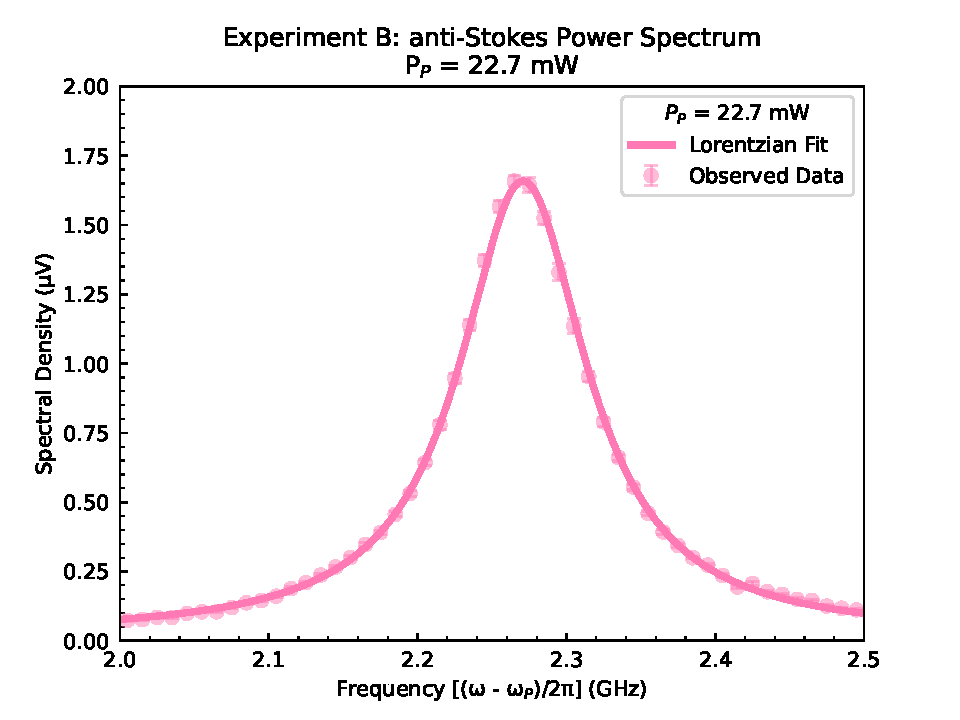
\includegraphics[width=\textwidth]{figs/2-Cooling/P-P anti-Stokes Fit - 55mW.pdf}
  \caption[Anti-Stokes probe spectra collected for \SI{22.7}{\milli\watt} intrafiber pump power in Experiment~B.]{Anti-Stokes probe spectra collected for \SI{22.7}{\milli\watt} intrafiber pump power in Experiment~B. Data is binned within \SI{10}{\mega\hertz} bins and displayed with error bars representing 1\(\sigma\) of spectral density. A Lorentzian fit has been computed based on the unbinned data and visual inspection confirms an excellent fit to the observed spectra. In conducting the experiment, five repeated measurements of both the anti-Stokes spectra and the background (pump off) were collected for each pump power, with each measurement comprising an average over 100 \SI{250}{\milli\second} sweeps at a \ac{RBW} of \SI{1}{\mega\hertz}. The spectral data shown here are the resulting background-subtracted spectra, with uncertainties propagated accordingly.}
  \label{fig:Cooling:P-P anti-Stokes Fit - 55mW}
\end{figure}

\begin{figure}[t!]
  \centering
  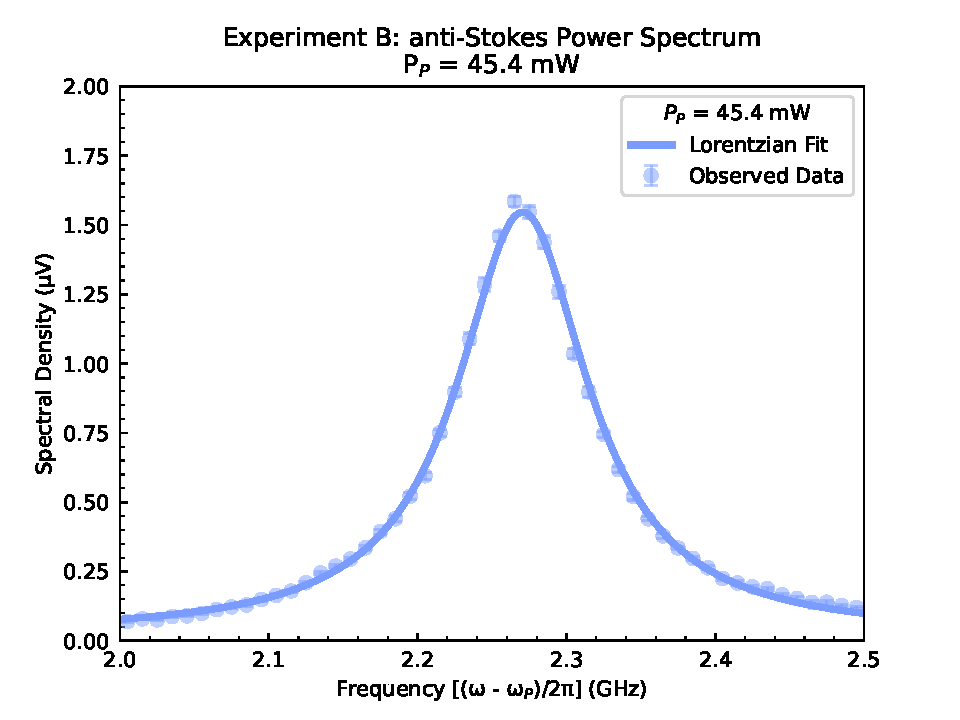
\includegraphics[width=\textwidth]{figs/2-Cooling/P-P anti-Stokes Fit - 110mW.pdf}
  \caption[Anti-Stokes probe spectra collected for \SI{45.4}{\milli\watt} intrafiber pump power in Experiment~B.]{Anti-Stokes probe spectra collected for \SI{45.4}{\milli\watt} intrafiber pump power in Experiment~B. Data is binned within \SI{10}{\mega\hertz} bins and displayed with error bars representing 1\(\sigma\) of spectral density. A Lorentzian fit has been computed based on the unbinned data and visual inspection confirms an excellent fit to the observed spectra. In conducting the experiment, five repeated measurements of both the anti-Stokes spectra and the background (pump off) were collected for each pump power, with each measurement comprising an average over 100 \SI{250}{\milli\second} sweeps at a \ac{RBW} of \SI{1}{\mega\hertz}. The spectral data shown here are the resulting background-subtracted spectra, with uncertainties propagated accordingly.}
  \label{fig:Cooling:P-P anti-Stokes Fit - 110mW}
\end{figure}

\begin{figure}[t!]
  \centering
  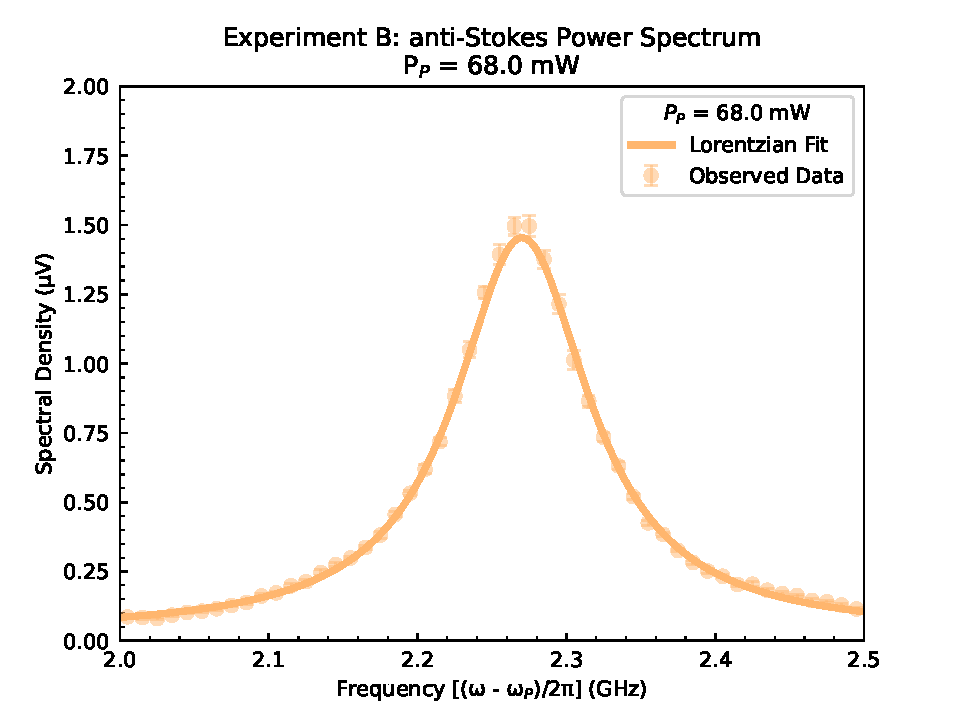
\includegraphics[width=\textwidth]{figs/2-Cooling/P-P anti-Stokes Fit - 165mW.pdf}
  \caption[Anti-Stokes probe spectra collected for \SI{68.0}{\milli\watt} intrafiber pump power in Experiment~B.]{Anti-Stokes probe spectra collected for \SI{68.0}{\milli\watt} intrafiber pump power in Experiment~B. Data is binned within \SI{10}{\mega\hertz} bins and displayed with error bars representing 1\(\sigma\) of spectral density. A Lorentzian fit has been computed based on the unbinned data and visual inspection confirms an excellent fit to the observed spectra. In conducting the experiment, five repeated measurements of both the anti-Stokes spectra and the background (pump off) were collected for each pump power, with each measurement comprising an average over 100 \SI{250}{\milli\second} sweeps at a \ac{RBW} of \SI{1}{\mega\hertz}. The spectral data shown here are the resulting background-subtracted spectra, with uncertainties propagated accordingly.}
  \label{fig:Cooling:P-P anti-Stokes Fit - 165mW}
\end{figure}

\begin{figure}[t!]
  \centering
  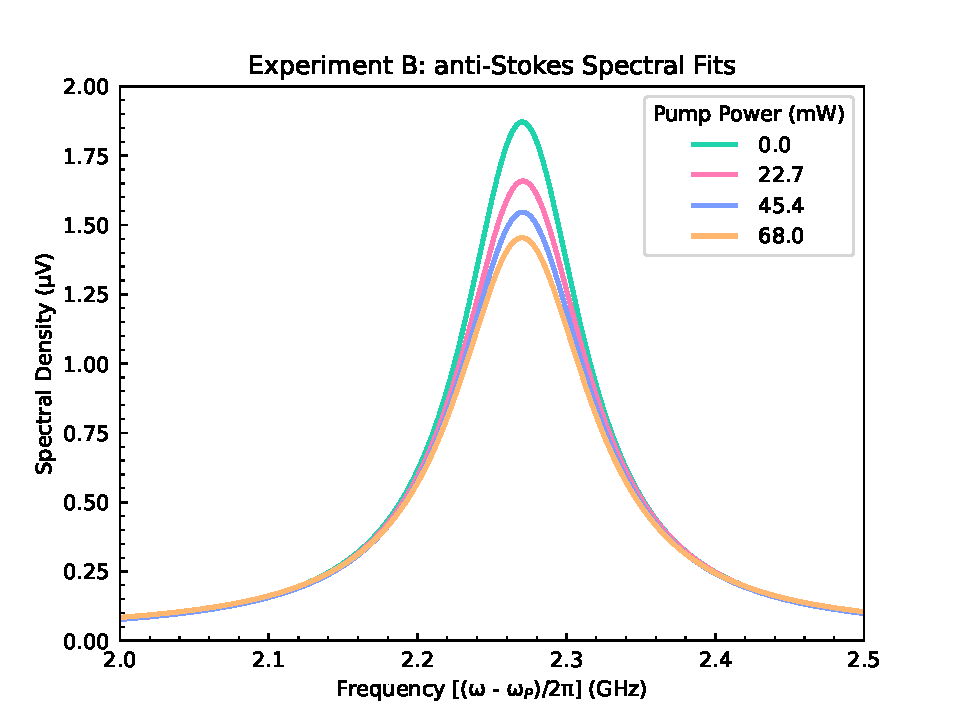
\includegraphics[width=\textwidth]{figs/2-Cooling/P-P anti-Stokes Fits.pdf}
  \caption[Computed Lorentzian fits from the observed anti-Stokes probe spectra gathered for Experiment~B.]{Computed Lorentzian fits from the observed anti-Stokes probe spectra gathered for Experiment~B, shown in Figures~\ref{fig:Cooling:P-P anti-Stokes Fit - 0mW}, \ref{fig:Cooling:P-P anti-Stokes Fit - 55mW}, \ref{fig:Cooling:P-P anti-Stokes Fit - 110mW}, and \ref{fig:Cooling:P-P anti-Stokes Fit - 165mW}, with consistent coloring across plots corresponding to intrafiber pump power. Fits are identical to those displayed with their respective observed spectra, with the fit parameters computed from the unbinned spectra for each intrafiber pump power. The decreasing trend in peak spectral density (proportional to phonon population) with increasing pump power (cooling) provides direct evidence of laser cooling of a band of traveling wave phonons within the \ac{LCOF}.}
  \label{fig:Cooling:P-P anti-Stokes Fits}
\end{figure}

\begin{figure}[t!]
  \centering
  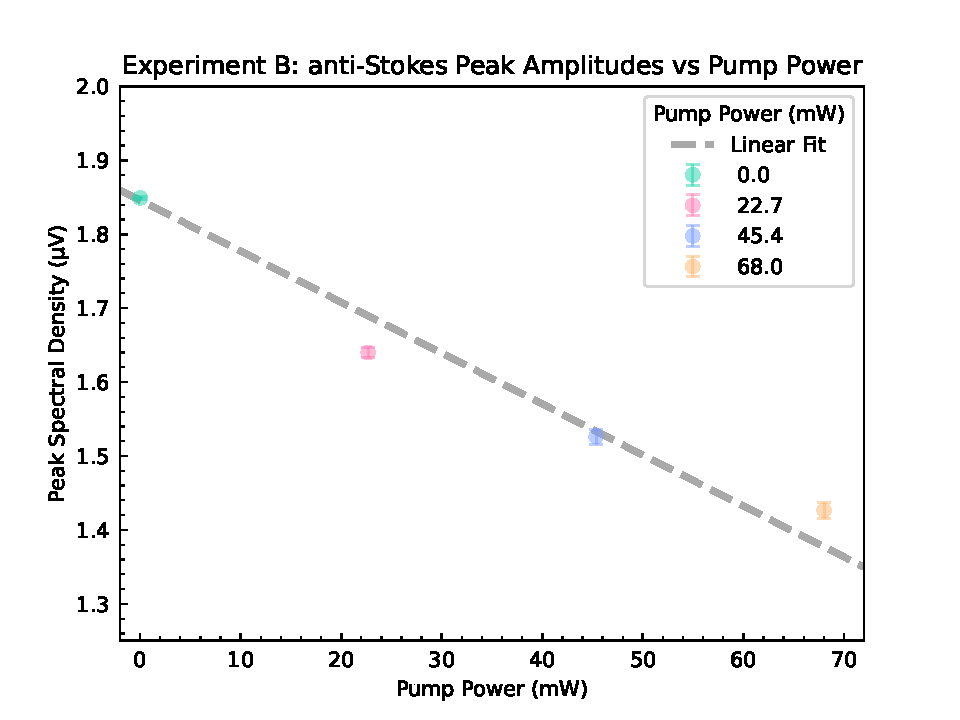
\includegraphics[width=\textwidth]{figs/2-Cooling/P-P anti-Stokes Height v Pow.pdf}
  \caption[Plot of peak spectral density amplitudes for the anti-Stokes spectra gathered for Experiment~B.]{Plot of peak spectral density amplitudes for the anti-Stokes spectra gathered for Experiment~B, corresponding to the four intrafiber pump powers used for the experiment. Values have been extracted from solved fit parameters for the Lorentzian fits displayed in Figure~\ref{fig:Cooling:P-P anti-Stokes Fits}, as well as individually with their respective observed spectra (Figures~\ref{fig:Cooling:P-P anti-Stokes Fit - 0mW}, \ref{fig:Cooling:P-P anti-Stokes Fit - 55mW}, \ref{fig:Cooling:P-P anti-Stokes Fit - 110mW}, and \ref{fig:Cooling:P-P anti-Stokes Fit - 165mW}). A linear fit has been applied to the data, showing a fair correlation to the data given the 1\(\sigma\) uncertainty representation for peak spectral density. The peak spectral amplitude is expected to decrease linearly with decreasing temperature of the mechanical mode due to anti-Stokes Brillouin cooling, consistent with Equation~\ref{eq:sponBSscatteredPower} for scattered power of the spontaneous Brillouin scattering process.}
  \label{fig:Cooling:P-P anti-Stokes Height v Pow}
\end{figure}

\begin{figure}[t!]
  \centering
  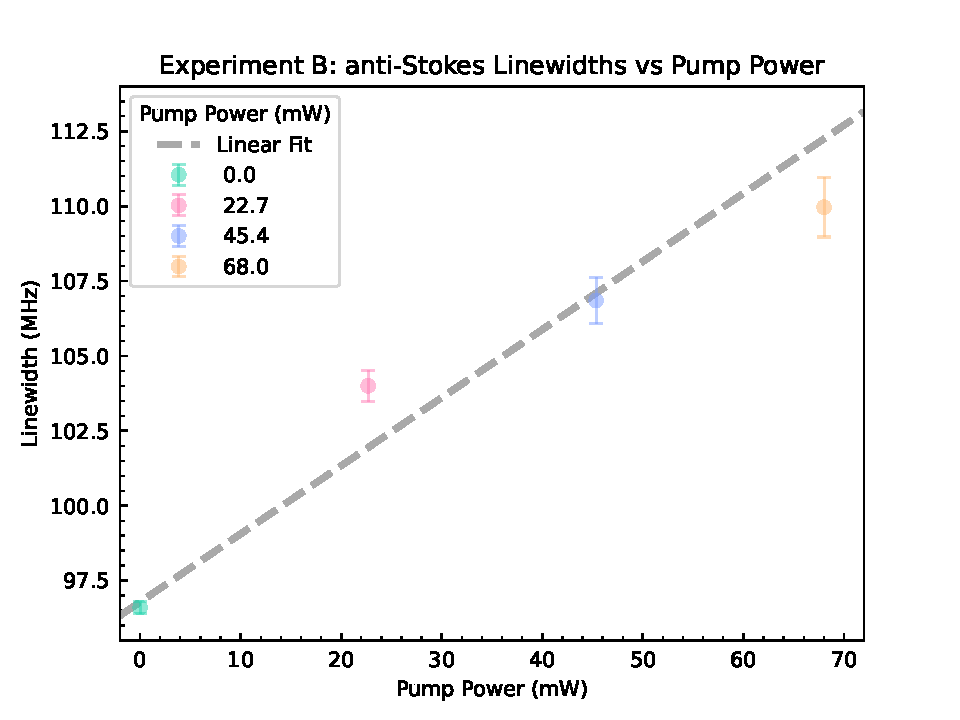
\includegraphics[width=\textwidth]{figs/2-Cooling/P-P anti-Stokes Wid v Pow.pdf}
  \caption[Plot of the \ac{FWHM} linewidths of the anti-Stokes spectra gathered for Experiment~B.]{Plot of the \ac{FWHM} linewidths of the anti-Stokes spectra gathered for Experiment~B, corresponding to the four intrafiber pump powers used for the experiment. Values have been extracted from solved fit parameters for the Lorentzian fits displayed in Figure~\ref{fig:Cooling:P-P anti-Stokes Fits}, as well as individually with their respective observed spectra (Figures~\ref{fig:Cooling:P-P anti-Stokes Fit - 0mW}, \ref{fig:Cooling:P-P anti-Stokes Fit - 55mW}, \ref{fig:Cooling:P-P anti-Stokes Fit - 110mW}, and \ref{fig:Cooling:P-P anti-Stokes Fit - 165mW}). A linear fit has been applied to the data, showing a fair correlation to the data, given the 1\(\sigma\) uncertainty representation for peak spectral density. Effective anti-Stokes linewidths are expected to increase linearly with increased pump power (cooling) according to Equation~\ref{eq:Cooling:effective linewidth}, absent pump depletion or any saturation effects. Discrepancies with a linear trend among the data presented with their associated vertical uncertainties are likely due to an underestimation of uncertainty in intrafiber pump power, which would be represented by some horizontal uncertainty associated with each data point. In the possible event of thermal saturation effects in the \ac{LCOF}, or unlikely pump depletion, we would expect to see linewidths exhibit a sublinear trend above a critical threshold of intrafiber pump power. While it is possible some minor saturation occured at these powers, a more conservative accounting of uncertainties in both linewidths and intrafiber pump powers is sufficient to explain a linear trend.}
  \label{fig:Cooling:P-P anti-Stokes Wid v Pow}
\end{figure}

\subsection{Evidence of Transmission Degradation}
\label{Cooling:subsec:Evidence of Transmission Degradation}

After comparing the anti‐Stokes linewidths measured in Experiments~A and B, we conclude that significant splice transmission degradation occurred in the interim. Experiment~B was performed first (with a through‐fiber transmission of 17\%), followed by Experiment~A the next day. If the experimental conditions were unchanged between the two experiments, the slopes of the anti‐Stokes linewidth versus pump power would be identical (Figures~\ref{fig:Cooling:P-O Linewidths} and \ref{fig:Cooling:P-P anti-Stokes Wid v Pow}). Instead, Experiment~B exhibits a noticeably steeper slope than Experiment~A. A reanalysis shows that reducing the assumed transmission for Experiment~A so the two slopes match would require the total fiber transmission to have dropped from 17\% down to approximately 3\%. While large, degradation of this level is plausible and is supported by several further points of analysis.

First, the optical performance of the splices bookending the \ac{LCOF}, already very delicate and suseptible to damage from nominal handling, are vulnerable to any particulates becoming lodged between the cores of the \ac{UHNA7} and \ac{LCOF}. While epoxy is among the more chemically resistant adhesives, any particulate contamination adhered to the surface of the epoxy or reservoire walls introduced from the environent during fabrication could easily become dislodged and settle into the splice opening. Some chemical dissolution of the epoxy within the reservoire by the \ce{CS2} after the prolonged soaking period (\SI{24}{\hour}) is also possible. Additionally, any unfortunate mechanical stress incurred during normal handling of the \ac{LCOF} is liable to cause damage and incur significant optical loss through one of the splices. Optical losses of this rate and magnitude, while not common, have been observed in several prior \ac{LCOF} samples.

Standard experimental procedure would catch this degradation in performance, however for this particular \ac{LCOF} sample, the exit fiber immediately following the end splice broke off irrepairably after testing its transmission, making it no longer possible to remeasure the full through‐fiber transmission during Experiment~A. In other words, if transmission had declined between experiments, we had no direct means of detecting it. Additionally, as seen in Figures~\ref{fig:Cooling:ExperimentADesign} and \ref{fig:Cooling:ExperimentBDesign}, the pump power was recorded prior to launch into the \ac{LCOF} for both experiments, providing no indication of change in performance of the splice between experiments. Hence, applying the same optical loss estimate to a splice that had experienced transmission degradation in the interim would have resulted in an overestimation of the actual power inside the \ac{LCOF} during Experiment~A (conducted after Experiment~B).

Further quantitative analysis supports this hypothesis as well. As we reported in Johnson et al. (2023), \cite{johnson2023laser} Experiment~A yields a Brillouin gain of approximately \SI{2.3}{\per\watt\per\meter}, calculated using Equation~\ref{eq:Cooling:effective linewidth}. This value is smaller than the \SI{6(1)}{\per\watt\per\meter} reported by Behunin et al. in 2019 \cite{behunin2019spontaneous} for a near‐identical \ac{LCOF} geometry and fabrication method. If instead we calculate the Brillouin gain based on the linewidths and corresponding intrafiber pump powers seen in the earlier Experiment~B, we find the Brillouin gain to be approximately \SI{8(2)}{\per\watt\per\meter}, which is in good agreement with the prior published value from the literature. In estimating the uncertainty here, we have taken the \(2\sigma\) confidence level in linewidths and allowed a 10\% uncertainty in intracore pump powers. The natural conclusion is that for Experiment~A we overestimated the intrafiber pump power due to the undetected splice transmission degradation between experiments. This produced an apparent smaller dependence of linewidth on pump power in Experiment~A and a consequent underestimation of the true gain of the \ac{LCOF}.

Finally, the linewidths of Experiment~B appear to exhibit a slight sublinear trend with power (Figure~\ref{fig:Cooling:P-P anti-Stokes Wid v Pow}), indicating the possibility of a saturation effect occuring at higher pump power. However any saturation effect or similar which could cause this trend should then also be activated at the higher pump powers used in Experiment~A, if the optical transmission were the same across experiments. If instead the transmission of the \ac{LCOF} entrance splice had been significantly greater for the earlier-run Experiment~B than for Experiment~A, the powers inside the \ac{LCOF} in Experiment~B could have been similar to or even greater than those in Experiment~A. This might explain why Experiment~B linewidths appear to exhibit slightly sublinear growth with pump power despite the lower pump powers launched into the \ac{LCOF} while Experiment~A does not seem to exhibit this same trend, despite the use of higher nominal pump powers. This is consistent with an estimated factor of 5 drop in transmission through the \ac{LCOF} splice between experiments, as indicated by the discrepancy in linewidth vs power slopes of each experiment.

In summary, all these lines of evidence strongly indicate that the \ac{LCOF} splice transmission fell substantially in the time between Experiments~B and A, by an approximate factor of five. This fully reconciles the differing slopes in the anti‐Stokes linewidth data and explains the otherwise surprising discrepancy in inferred Brillouin gain compared to values published in the literature for identical \ce{CS2}-filled \ac{LCOF}s. This conclusion implies even higher performance of our \ac{LCOF} example than was previously understood and reported in Johnson et al. (2023): \cite{johnson2023laser} the amount of cooling achieved (unaffected by this reanalysis) was accomplished with far less pump power.

%--------------------------------------------------------------------%

\section{Discussion}
\label{Cooling:sec:Discussion}

\subsection{The C-Value: A Standardized Cooling Metric}
\label{Cooling:subsec:StandardizedCoolingMetric}

Cooling results are often reported in degrees kelvin cooled, sometimes only implicitly stated from room temperature. While this is understood by researchers closely following laser cooling, it can be misleading to those who are looking to apply these published techniques to systems not starting at room temperature. A lack of clarity of cooling performance as being a function of starting temperature may cause buyer's remorse among researchers who expend resources to employ the technique only to realize less than advertised absolute degrees cooling of a material below room temperature. Even for the more careful researcher this introduces frustration in the literature review process. To address this, we propose a normalized cooling metric be adopted to report the fractional degrees cooled relative to initial temperature. We introduce the \emph{\ac{C}}, or \emph{C-value}, expressed as a percentage of degrees cooled from initial temperature,

\begin{equation}
  C = \frac{\Delta T}{T_{0}}.
\end{equation}
\\
Reporting the \(C\)-value of a cooling technique offers greater transparency, clarity, and universal applicability of performance across cooling techniques and application fields. Recent discussions in the optical refrigeration community have similarly called for standardized cooling metrics to ensure fair, reproducible comparisons of cooling results. \cite{zhang2024experimental} Indeed, reporting only absolute degrees cooled may significantly \emph{under}represent the performance of a given technique if applied to a material above room temperature (as is often the case for data center and information processing applications \cite{}). Adopting the \(C\)-value for cooling performance will expand the perceived viability and utility of laser cooling techniques to researchers outside of optomechanical physics and related fields, potentially spurring greater investment interest in the advancement of laser cooling techniques. As such, we report a \(C\)-value of 12\%, achieved with \SI{68.0}{\milli\watt} of intrafiber pump power (Experiment~B).

By contrast, the recent result by Martinez et al. (Max Planck Institute, 2024) \cite{blazquez2024optoacoustic} demonstrated a much larger \(\Delta T \approx\) \SI{219}{\kelvin} cooling from room temperature, an unprecedented \(C\)-value of 73\% cooling of the phonon mode’s temperature. This emphasizes the Max Planck group’s achievement of removing nearly three-quarters of the thermal energy from that acoustic mode, a level on par with the best solid-state optical cryocoolers, which have reached \(\sim\)\SI{91}{\kelvin} from ambient (\(\sim\)70\% cooling) in Yb-doped crystals. \cite{zhang2024experimental} The fractional metric thus allows us to compare techniques across disparate systems such as optical fibers and bulk crystals on equal footing for their cooling effectiveness. As approaches push toward lower starting temperatures (e.g. pre-cooled or cryogenic environments), absolute \(\Delta T\) naturally shrinks, but a high \(C\)-value will remain notable. Adopting the \(C\)-value, in combination with a commitment to publishing sufficiently rigorous experimental context, \cite{zhang2024experimental} yields a transparent gauge of performance across diverse temperature regimes and material platforms.

\subsection{Parallel Achievement: Max Planck Institute}
\label{Cooling:subsec:Parallel Achievement}

The principles demonstrated in this chapter can be directly compared to parallel work by other groups using different fiber platforms. In particular, Martinez et al. (2024) \cite{blazquez2024optoacoustic} reported optoacoustic cooling of traveling phonons in a tapered chalcogenide \ac{PCF}. In their experiment, a \SI{50}{\centi\meter} long PCF with a microstructured, tapered core was used to enhance optomechanical coupling. Like our system, the Max Planck group employed Brillouin backscattering in a continuous waveguide to achieve phonon cooling of traveling-wave phonons. The underlying mechanism is the same: anti-Stokes scattering removes thermal phonons by converting them into higher-energy photons that promptly leave the system. Both platforms therefore rely on traveling-wave Brillouin interactions and leverage the fast escape of anti-Stokes light compared to phonon thermalization times to cool a band of acoustic modes.

Despite these similarities in principle, there are important differences in the experimental implementation. The \ac{PCF} platform uses a solid chalcogenide fiber with a patterned microstructure, which was tapered to a small core diameter. The combined material and geometric parameters yield an acoustic mode at \SI{7.38}{\giga\hertz} (higher than the \SI{2.27}{\giga\hertz} acoustic band in our liquid-core fiber) and a very large effective Brillouin gain coefficient \(G_{\rm B} \sim\)\SI{180}{\per\watt\per\meter}. The higher acoustic frequency in the \ac{PCF} means each phonon carries more energy (\(\hbar\Omega_{\rm B}/k_{\rm B} \approx\) \SI{0.35}{\kelvin} vs \SI{0.1}{\kelvin} for our system), but also that the mean thermal occupation at room temperature is lower (on the order of \(10^{2}\) vs. a \(10^{3}\) in our lower frequency mode). The two experiments also operated at different pump power: our work used a modest \SI{68.0}{\milli\watt} of laser power to achieve \SI{35}{\kelvin} of cooling (Experiment~B), whereas the \ac{PCF} results employed a maximum pump power of nearly \SI{250}{\milli\watt} to achieve the reported \SI{219}{\kelvin} cooling from room temperature, or a \(C\)-value of 74.7\%. \cite{blazquez2024optoacoustic}

\subsection{Pathways to Net Cooling}
\label{Cooling:subsec:PathwaystoNetCooling}

While the experiments to date (including this work and Martinez et al.) achieve cooling of a phonon mode relative to the ambient lattice temperature, the phonon population of the overall system remains uncooled due to the inverse process (Stokes) simultaneously depositing energy into the Stokes phonon mode. Net cooling would imply extracting heat faster than it is replenished by both thermalization (the natural dissipation rate of the system) \emph{and} Stokes scattering of the Stokes phonon mode. Engineering a system to reach this regime is a challenge, but we envision several pathways that could tip the balance toward net cooling.

One strategy is to bias the gain in favor of anti-Stokes scattering within a single transit of the medium, by suppressing or preventing Stokes processes through waveguide design. In a standard fiber, any pump photon has some probability to scatter into a Stokes photon, creating a phonon, which counteracts cooling. If we can reduce the likelihood of Stokes scattering while allowing anti-Stokes scattering to proceed, the net effect in one pass will be phonon removal without equivalent phonon creation. For example, one could design a fiber or waveguide that does not efficiently guide the Stokes-shifted wavelength, similar to a photonic bandgap fiber that places the Stokes frequency in a bandgap. In such a fiber, a pump photon could still undergo anti-Stokes scattering, but a would-be Stokes photon falls outside the guided modes and is effectively not generated.

Another approach is to incorporate an out-of-plane coupling mechanism to an absorbing medium or a frequency cutoff for only the Stokes. By asymmetrically enhancing loss for Stokes, one can bias the single-pass Brillouin interaction toward net phonon annihilation. By diverting the Stokes field away from the guided mode through an engineered out-of-plane coupling, we can effectively “dump” the Stokes into a loss channel while preserving the anti-Stokes within the waveguide core, thus favoring net phonon removal. For instance, one might introduce a side-etched structure or grating that phase-matches only to the Stokes frequency, routing Stokes photons into an absorbing or radiative mode. Meanwhile, the anti-Stokes remains confined to the original waveguide, continuing to interact with the target phonon mode. Such a design ensures that Stokes photons, once generated, are immediately evacuated before they can drive the reverse (phonon creation) process. When combined with sufficiently strong anti-Stokes gain, this asymmetric loss channel could break the symmetry of phonon creation and annihilation within a single transit, thereby accelerating phonon cooling. Although this approach demands precise control over waveguide geometry and materials to selectively scatter and absorb Stokes without degrading anti-Stokes propagation, it holds promise for realizing net cooling in practical fiber architectures.

Another promising avenue for enhancing net phonon cooling in continuous Brillouin systems is the deliberate engineering of a group-velocity bias between the Stokes and anti-Stokes waves. By differentiating their propagation speeds, one introduces a temporal asymmetry in interaction strength that preferentially enables phonon annihilation over phonon creation. Some works explore this idea via enhancement of the optical density-of-states at the anti-Stokes frequency via slow-light or resonance effects while reducing it at the Stokes frequency. \cite{kim2017role, bahl2012observation} Crucially, however, any group velocity bias strategy must be designed with the phonon lifetime and effective system length in mind, as effective cooling demands that anti-Stokes photons carry away energy faster than the phonon mode thermally repopulates.

\subsection{Applications to Ground State Cooling}
\label{Cooling:subsec:ApplicationstoGroundStateCooling}

Reaching lower phonon occupancies and ultimately approaching the quantum ground state of a traveling acoustic wave mode is not only a scientific milestone but also an enabling step for quantum applications. Cooling traveling-wave phonons toward the ground state means drastically reducing their thermal noise, to the point that quantum mechanical effects of the phonons emerge. In the quantum regime, a traveling acoustic phonon mode in an optical fiber can serve as a memory or intermediary for quantum states of light. Photons can be coherently converted to phonons and back, effectively storing the photonic state in a mechanical degree of freedom. Coupling light to acoustic phonons has already been used to demonstrate all-optical signal storage and delay in classical contexts. For example, light pulses can be fully converted into acoustic waves and retrieved after a storage interval. \cite{merklein2017chip} If those acoustic waves are in a near-ground-state (low-noise) condition, one could perform the same feat at the single-photon level, realizing a broadband quantum memory at telecom wavelengths. Such a memory would be reversible and coherent, capable of storing quantum information (amplitude and phase of a single-photon wavepacket) for microsecond durations. \cite{merklein2017chip} Moreover, a low-phonon-temperature waveguide could function as a quantum optical delay line or buffer with minimal added noise, preserving quantum states during the delay.

If the traveling acoustic mode approaches its ground state, one can begin to prepare and manipulate non-classical phonon states. This could include generating single phonons on demand, phonon Fock states, or entangled states between phonons and photons. One exciting prospect is creating entangled states between a traveling phonon and a propagating photon. The cooled phonon mode would have low enough noise to allow high-fidelity entanglement generation via stimulated scattering processes. In fact, a recent proposal by Zhu et al. (2024) suggests that even without ground-state preparation, one can generate entangled photon–phonon pairs in a fiber using pulsed Brillouin processes. \cite{zhu2024optoacoustic} Their scheme relies on a two-pump configuration to create correlated Stokes and anti-Stokes photons along with a phonon, and remarkably it does not require the phonon to start in the ground state. If the phonon mode were already near its ground state, one can imagine the entanglement rates and purity could be even higher. Beyond two-party entanglement, could facilitate multi-mode quantum state engineering, for example, creating squeezed phonon states. \cite{hu1996squeezed} The ability to manipulate a continuum of phonon modes at the quantum level might also enable quantum acoustic signal processing, where information is encoded in phononic wavepackets and processed (filtered, delayed, interfered) with quantum coherence. \cite{manenti2017circuit}

Achieving ground-state cooling of a macroscopic, traveling-wave phonon mode will likely require a hybrid approach: combining conventional cryogenics with our laser cooling techniques. Cavity optomechanics experiments regularly precool the device to liquid helium temperatures before applying laser cooling to reach the quantum ground state, \cite{doeleman2023brillouin} and the same idea applies to continuous systems. Placing the optical fiber or waveguide in a cryostat lowers the baseline phonon occupancy, dramatically reducing the gap to the ground state. Laser cooling could then be applied to overcome the remaining thermal quanta.

\subsection{Conclusion}
\label{Cooling:subsec:Conclusion}

In conclusion, the work presented in this chapter establishes a robust foundation for fiber-based optomechanical cooling of traveling-wave phonons, pushing the boundaries of what can be achieved in continuous-wave Brillouin systems. By demonstrating Brillouin anti-Stokes cooling in a carefully engineered \ac{LCOF} platform, we have shown that laser cooling need not be relegated to highly specialized chip waveguides or microresonators. The advantageous optomechanical properties of the \ac{LCOF} enabled clear evidence of laser cooling under ambient conditions and marks the first demonstration of its kind in a fiber format. This proof of principle opens up numerous opportunities for fiber-based applications, including precision metrology, low-noise acousto-optic devices, and quantum information schemes requiring mechanically cooled states. By demonstrating the capacity to cool traveling-wave phonons in an optical fiber, this work lays the groundwork for future low-noise photonic devices and advanced acousto-optic technologies, marking a significant step toward quantum-limited acoustic control.

\clearpage
\thispagestyle{empty}
\null
\newpage
